\section{Extra figures}
\subsection{Experiments on Corrupted datasets}
\label{app:t2c}
\begin{figure}[H]
    \centering
    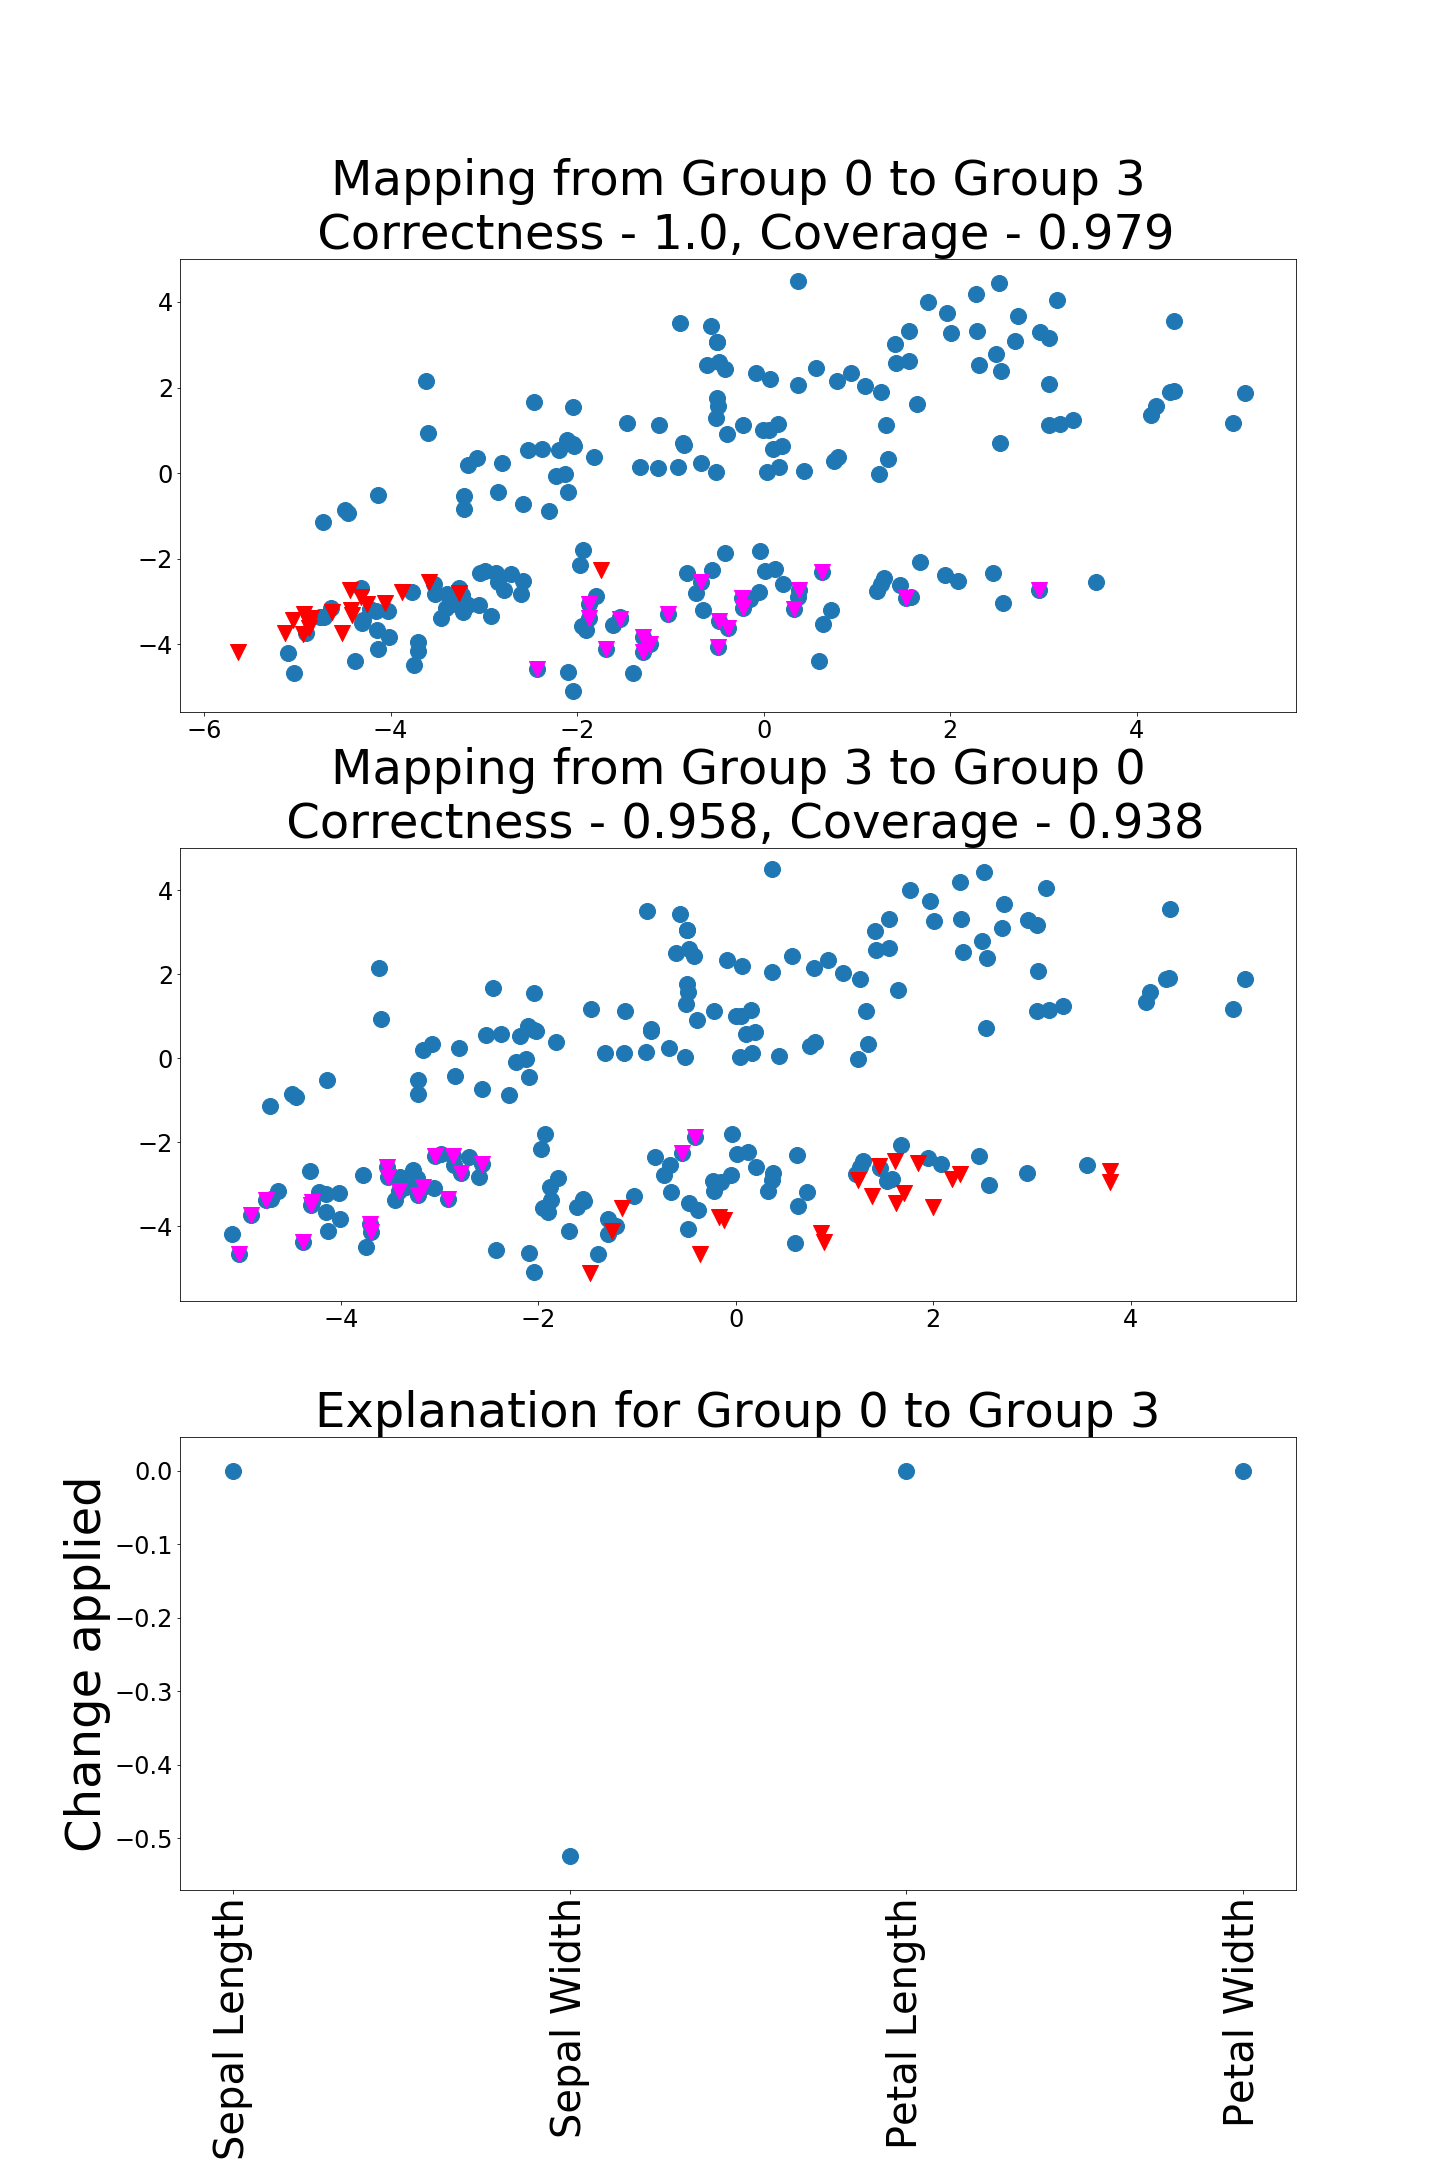
\includegraphics[width=0.4\textwidth, height=7.2cm]{../openreview/images/tffigures/iris-t2c.png}
    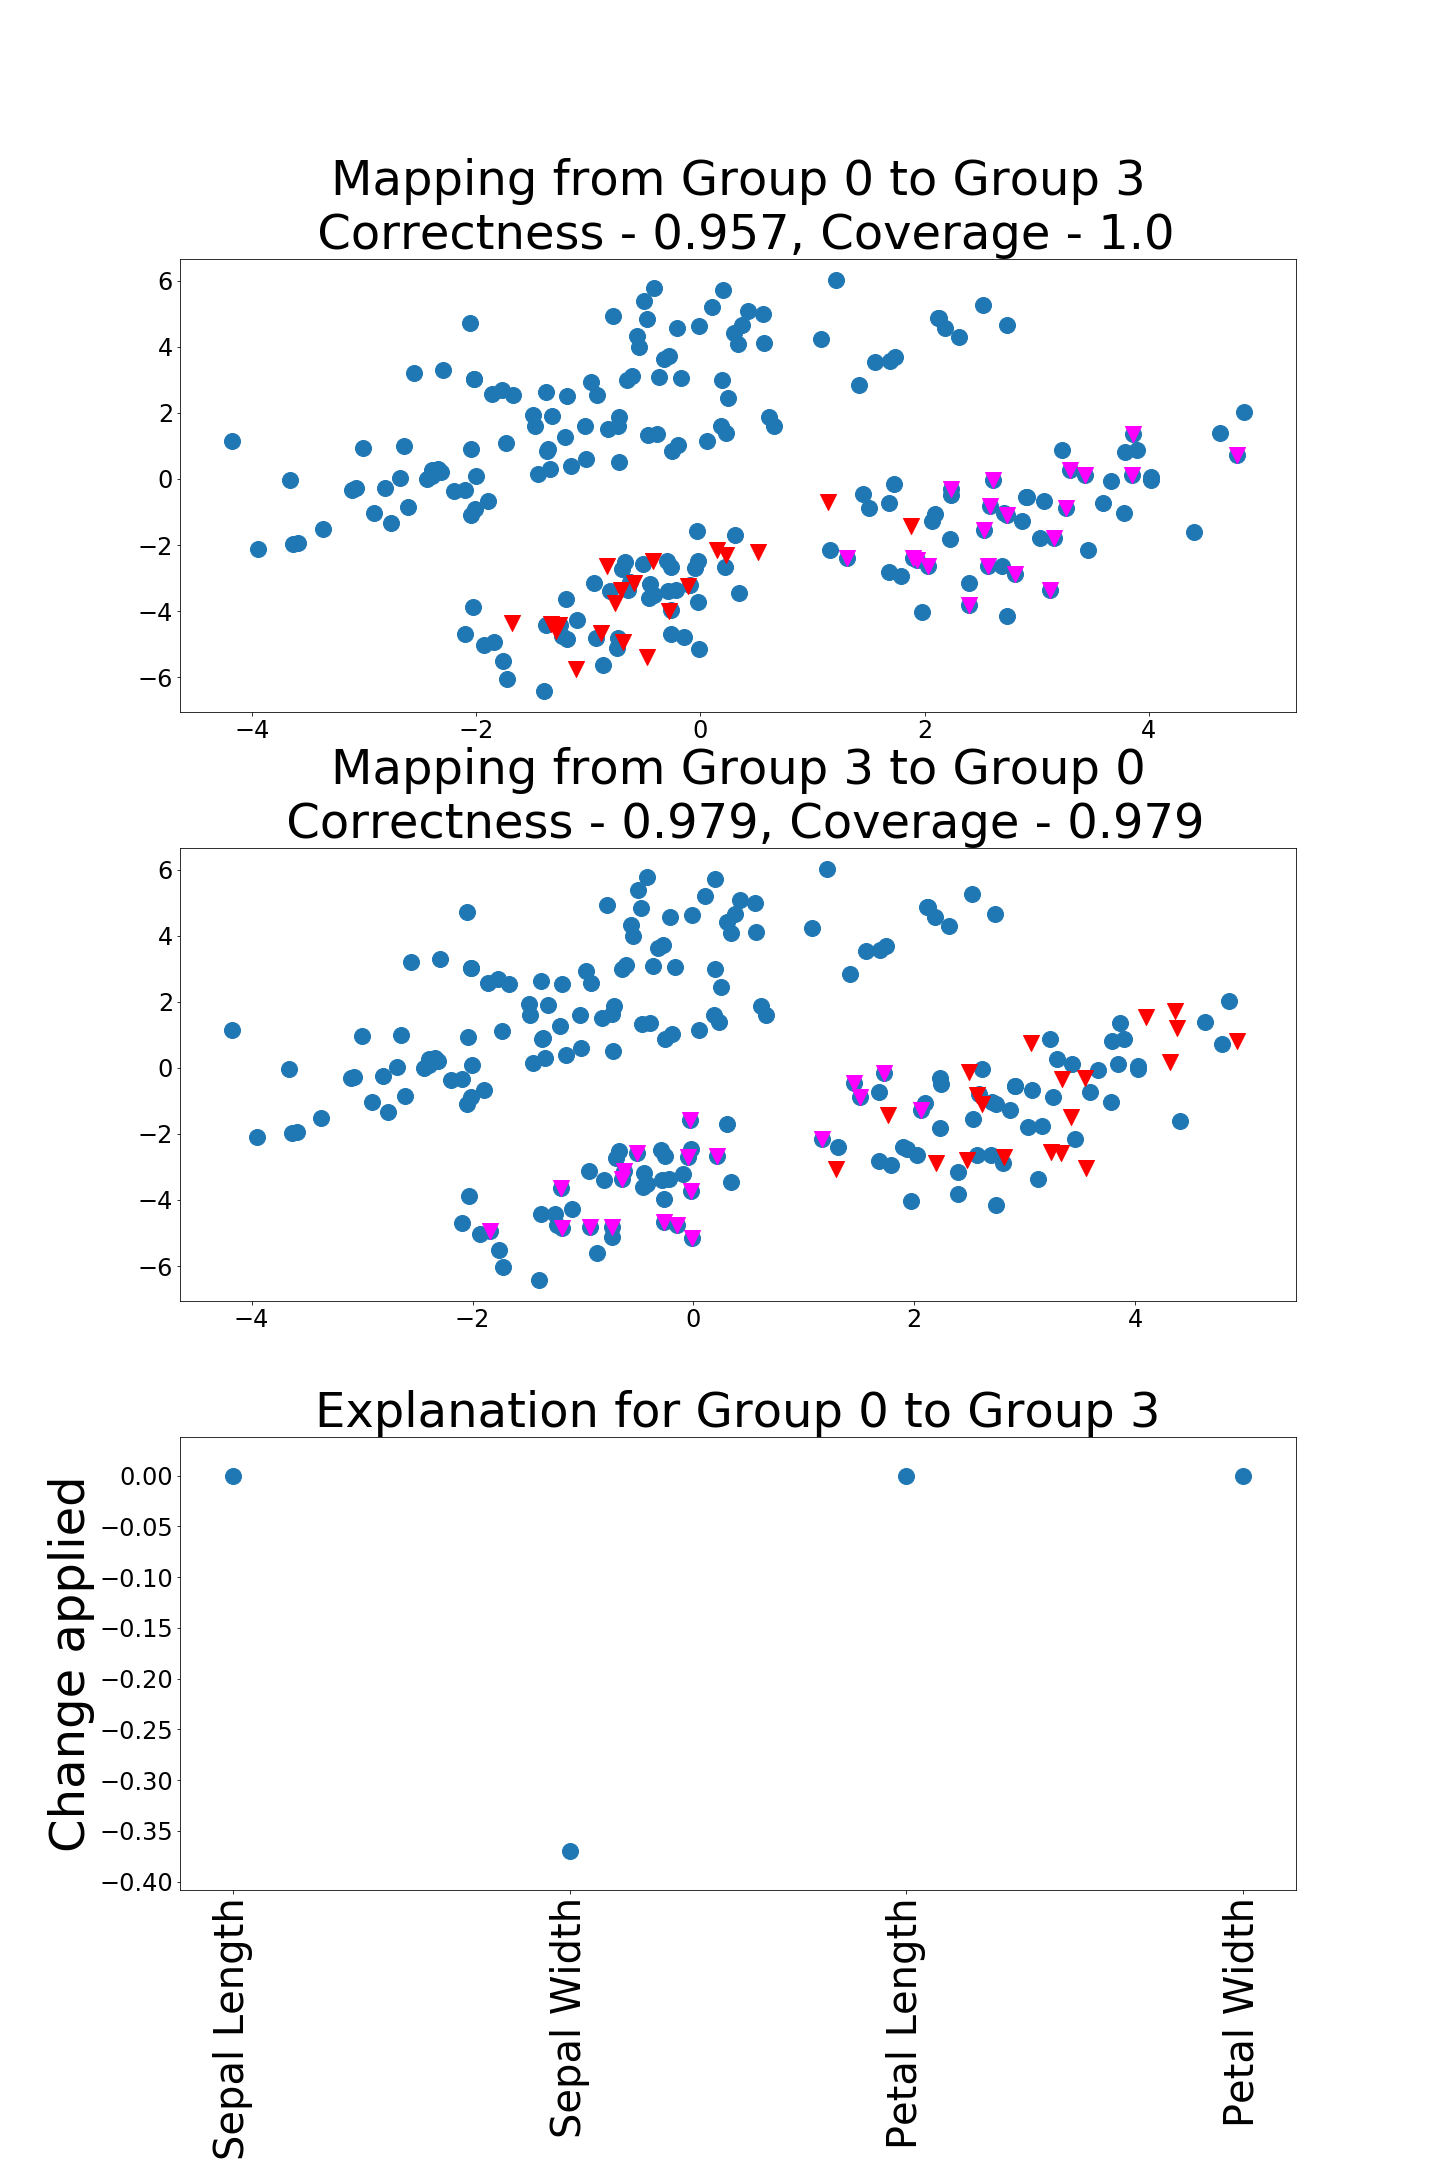
\includegraphics[width=0.4\textwidth, height=7.2cm]{../openreview/images/tffigures/iris-retrained-t2c.png}
    \caption{Explanation for corrupted features on UCI Iris dataset. Feature modified is 1(Sepal Width). Left: Visualization of the TGT explanations on the modified dataset. Right: Visualization of the TGT explanations with scVIS retrained on the modified dataset. We observe that the TGT explanations are robust to the modifications.}
    \label{fig:t2c-Iris}
\end{figure}
\begin{figure}[H]
\centering
    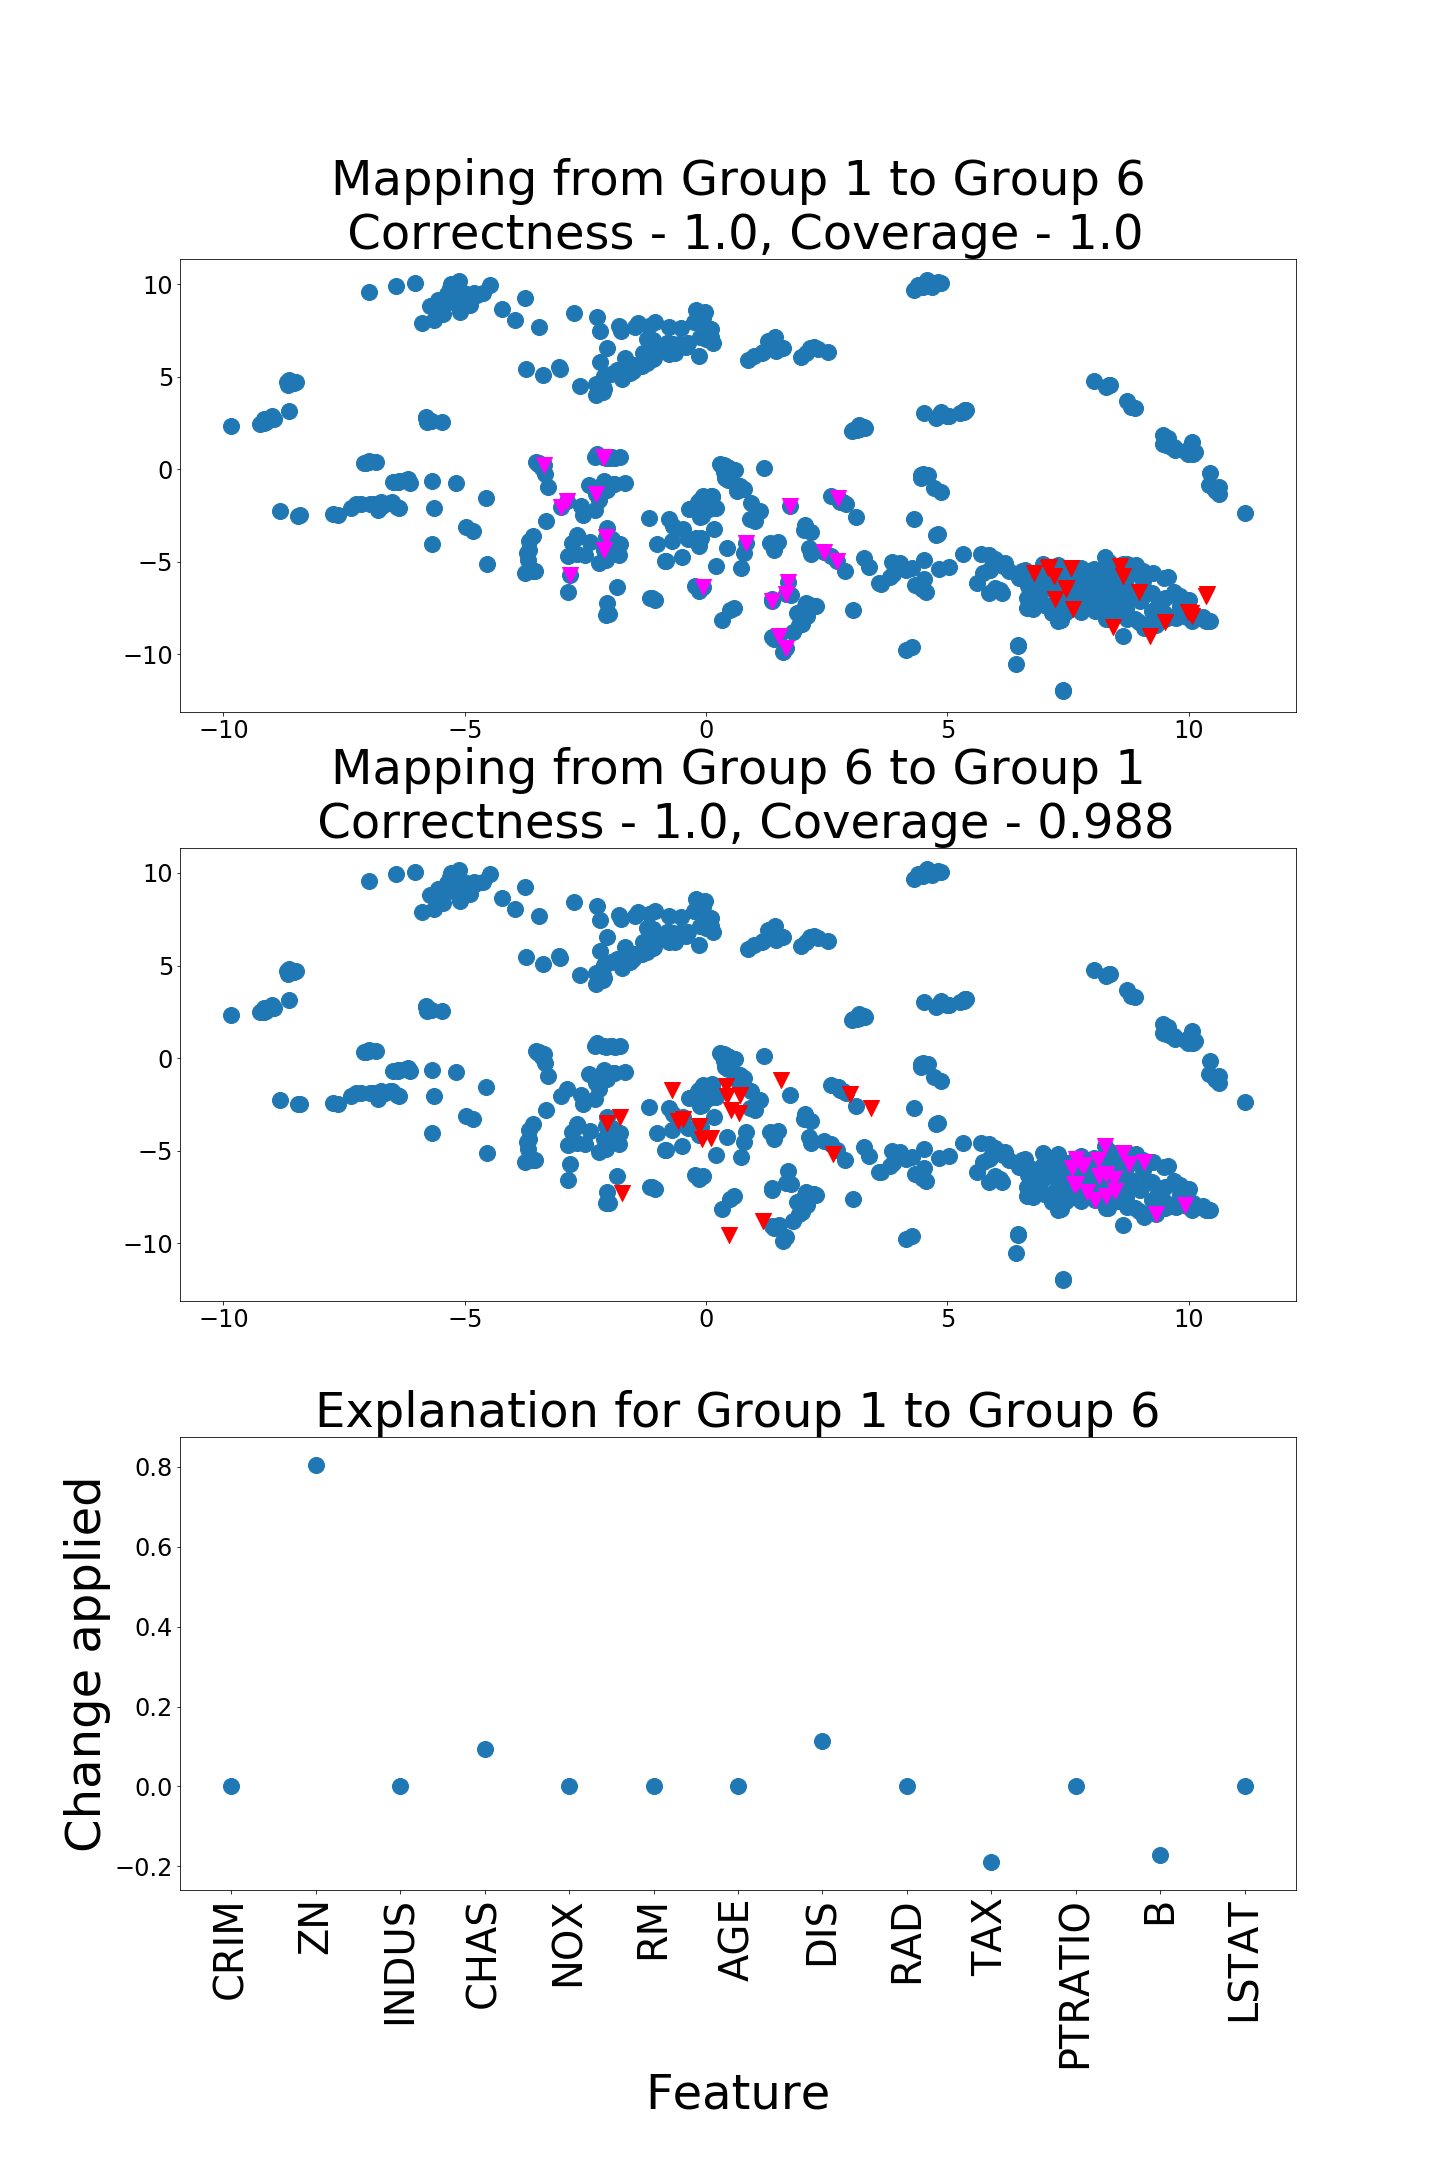
\includegraphics[width=0.4\textwidth, height=7.2cm]{../openreview/images/tffigures/housing-t2c.png}
    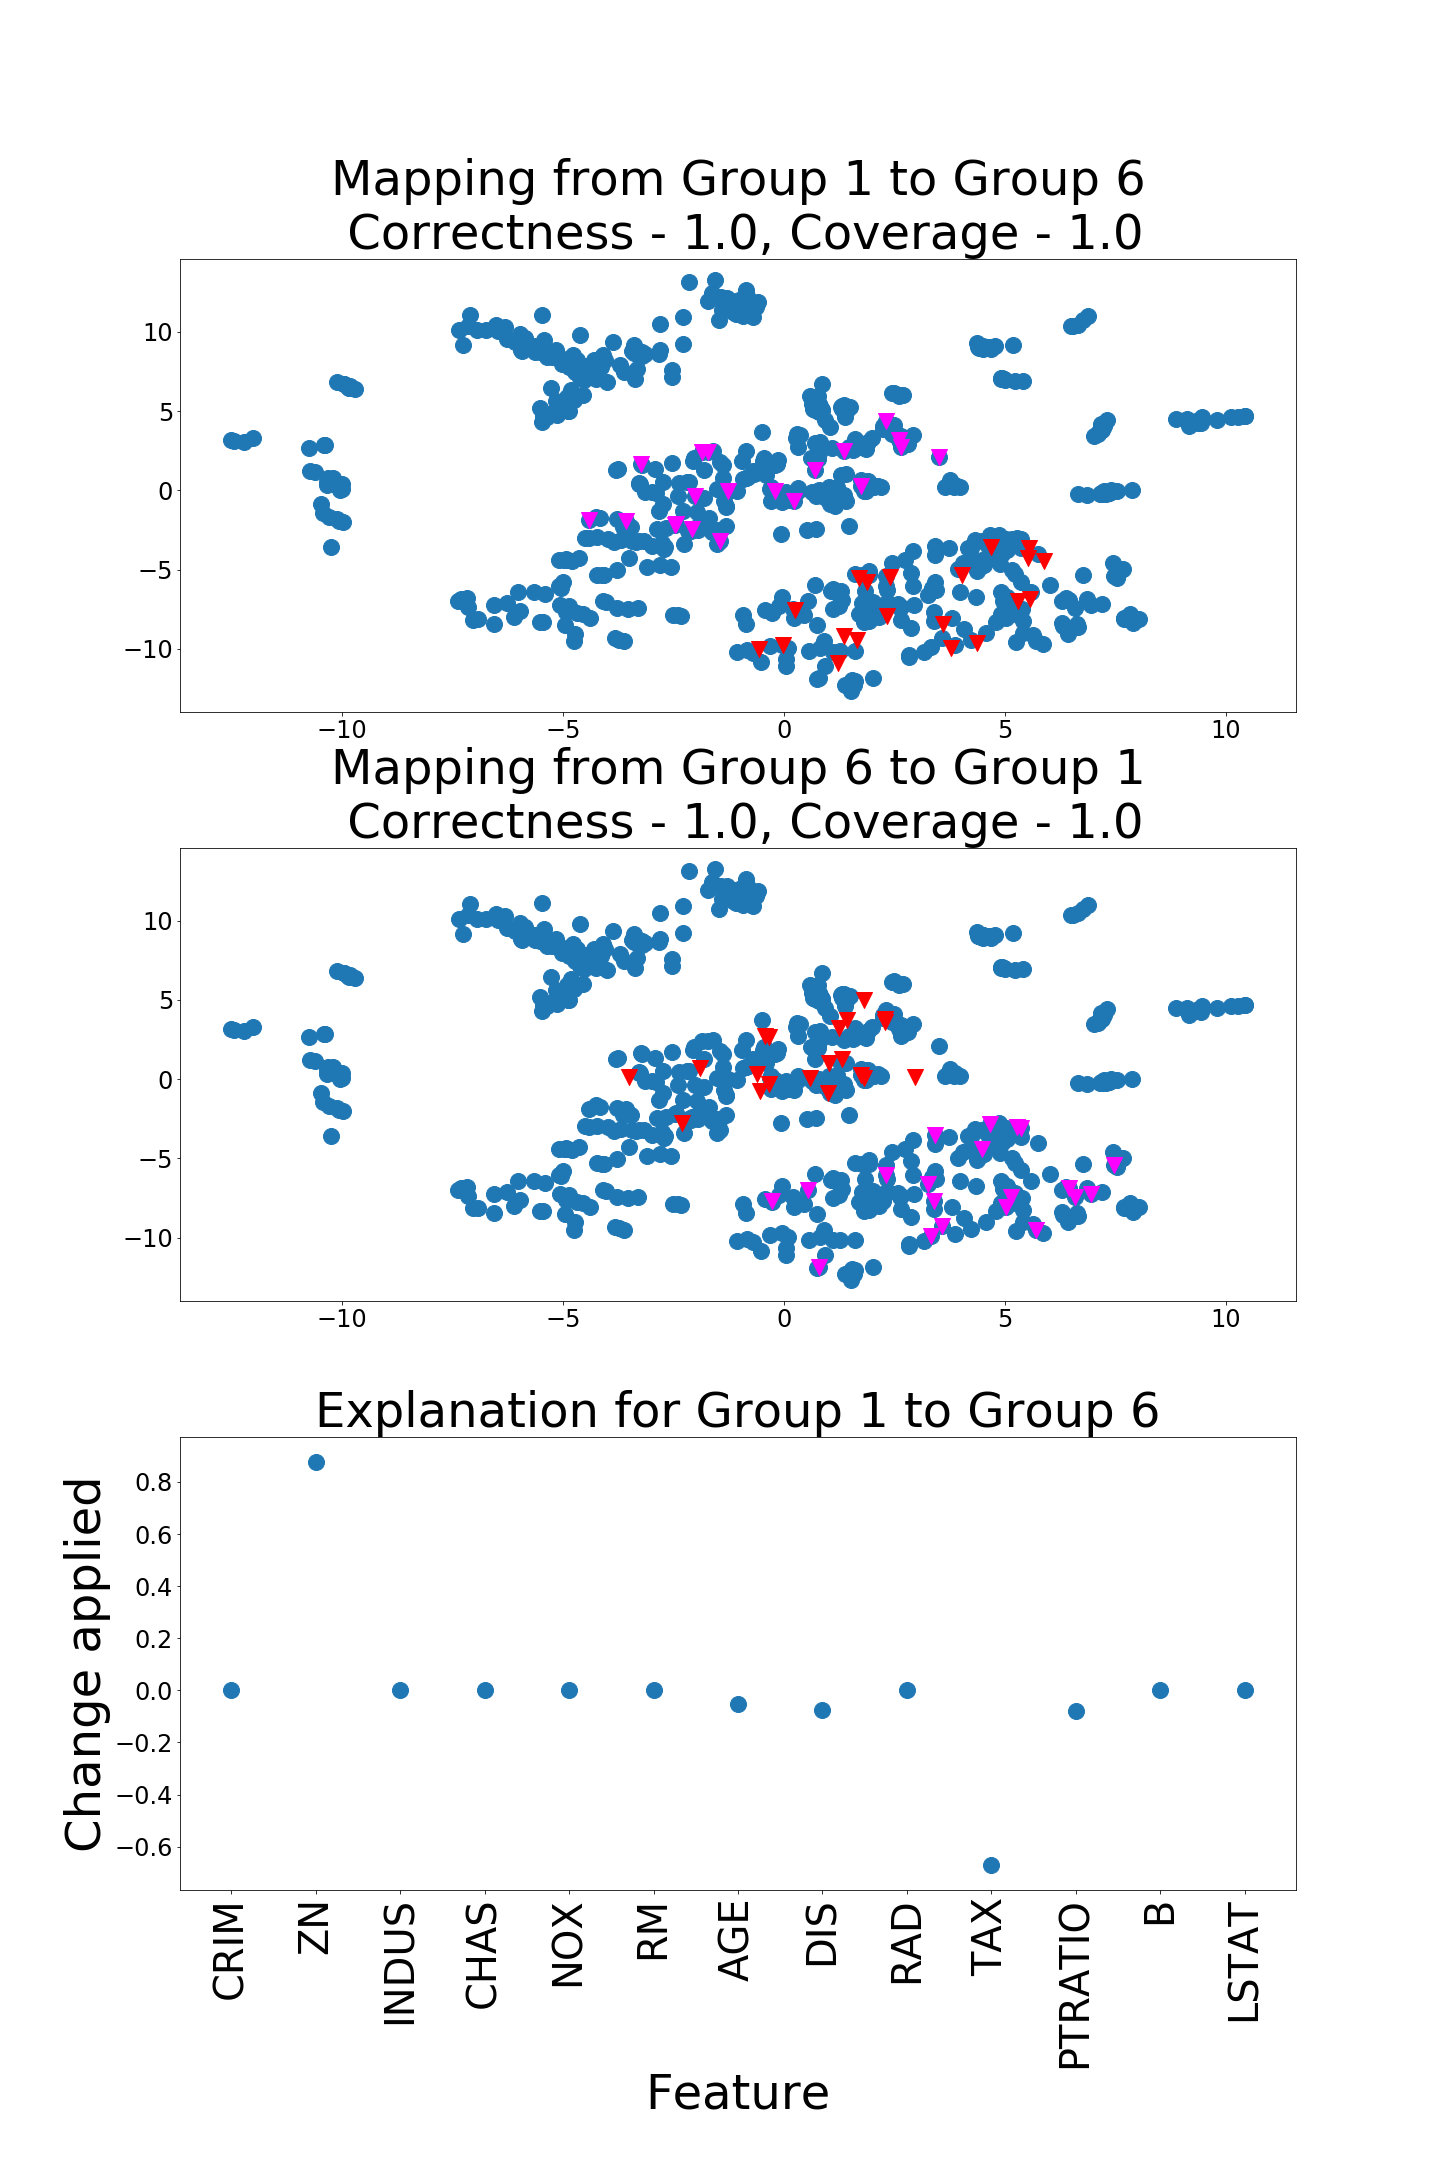
\includegraphics[width=0.4\textwidth, height=7.2cm]{../openreview/images/tffigures/housing-retrained-t2c.png}
    \caption{Explanation for corrupted features on UCI Boston Housing dataset. We modify the features 1(ZN) and 9(TAX). Left: Visualization of the TGT explanations on the modified dataset. We observe that TGT returns noisy explanations in this case. Right: Visualization of the TGT explanations with scVIS retrained on the modified dataset. With retrained scVIS model, TGT is able to recover the modifications.}
    \label{fig:t2c-Housing}
\end{figure}
\begin{figure}[H]
    \centering
    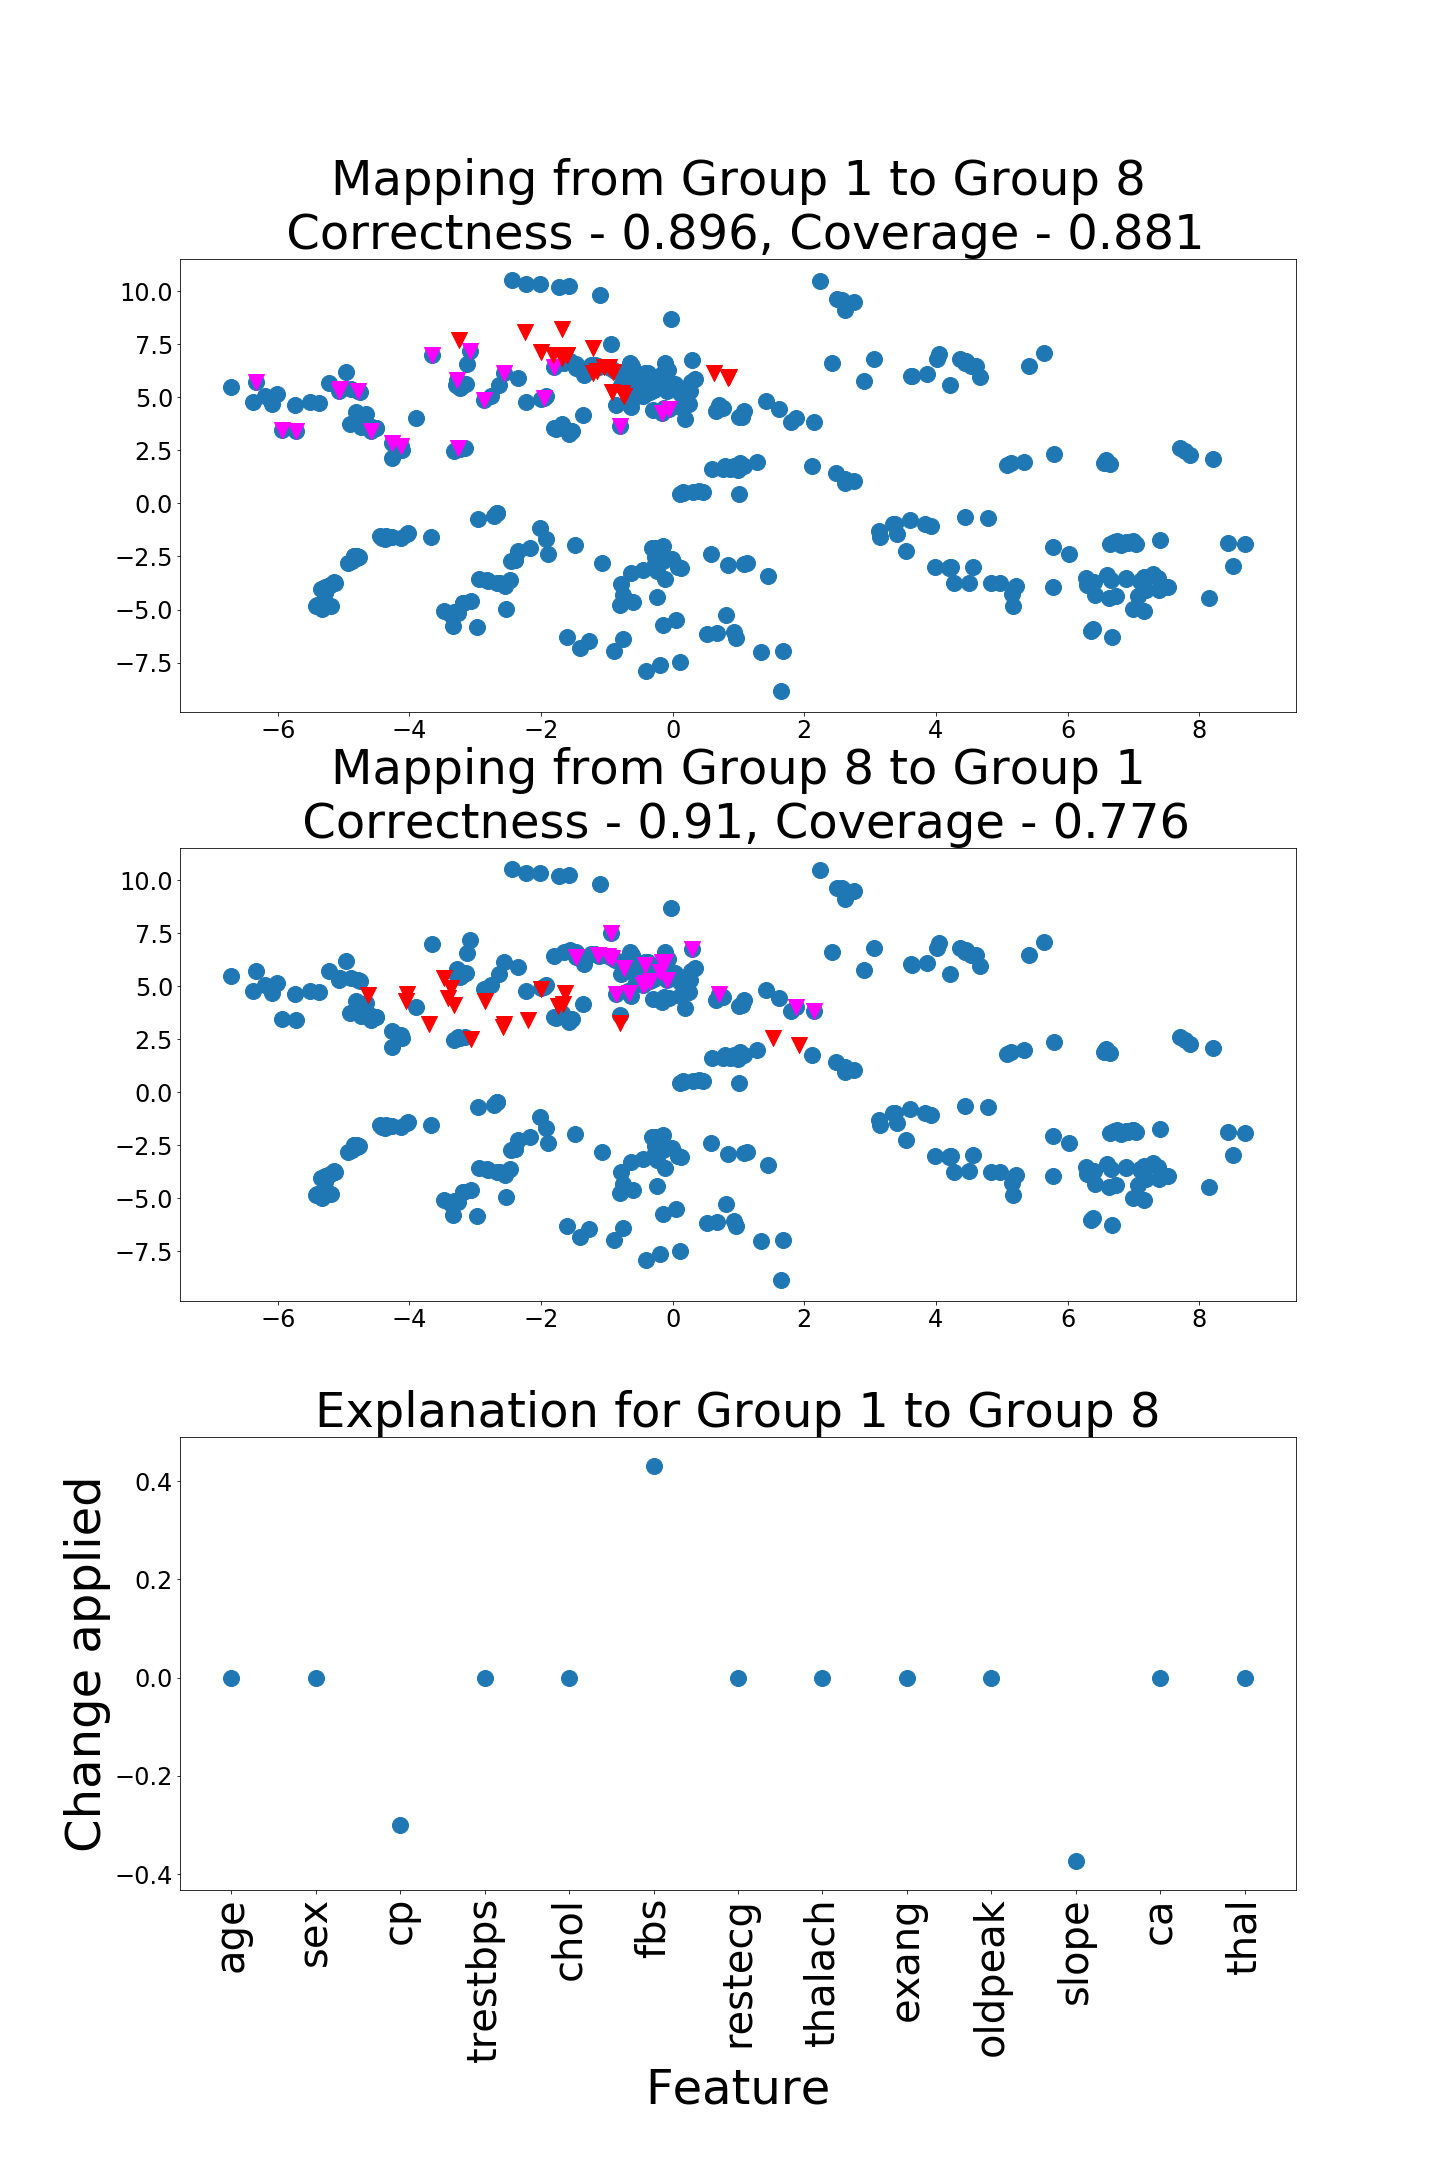
\includegraphics[width=0.4\textwidth, height=7.2cm]{../openreview/images/tffigures/heart-t2c.png}
    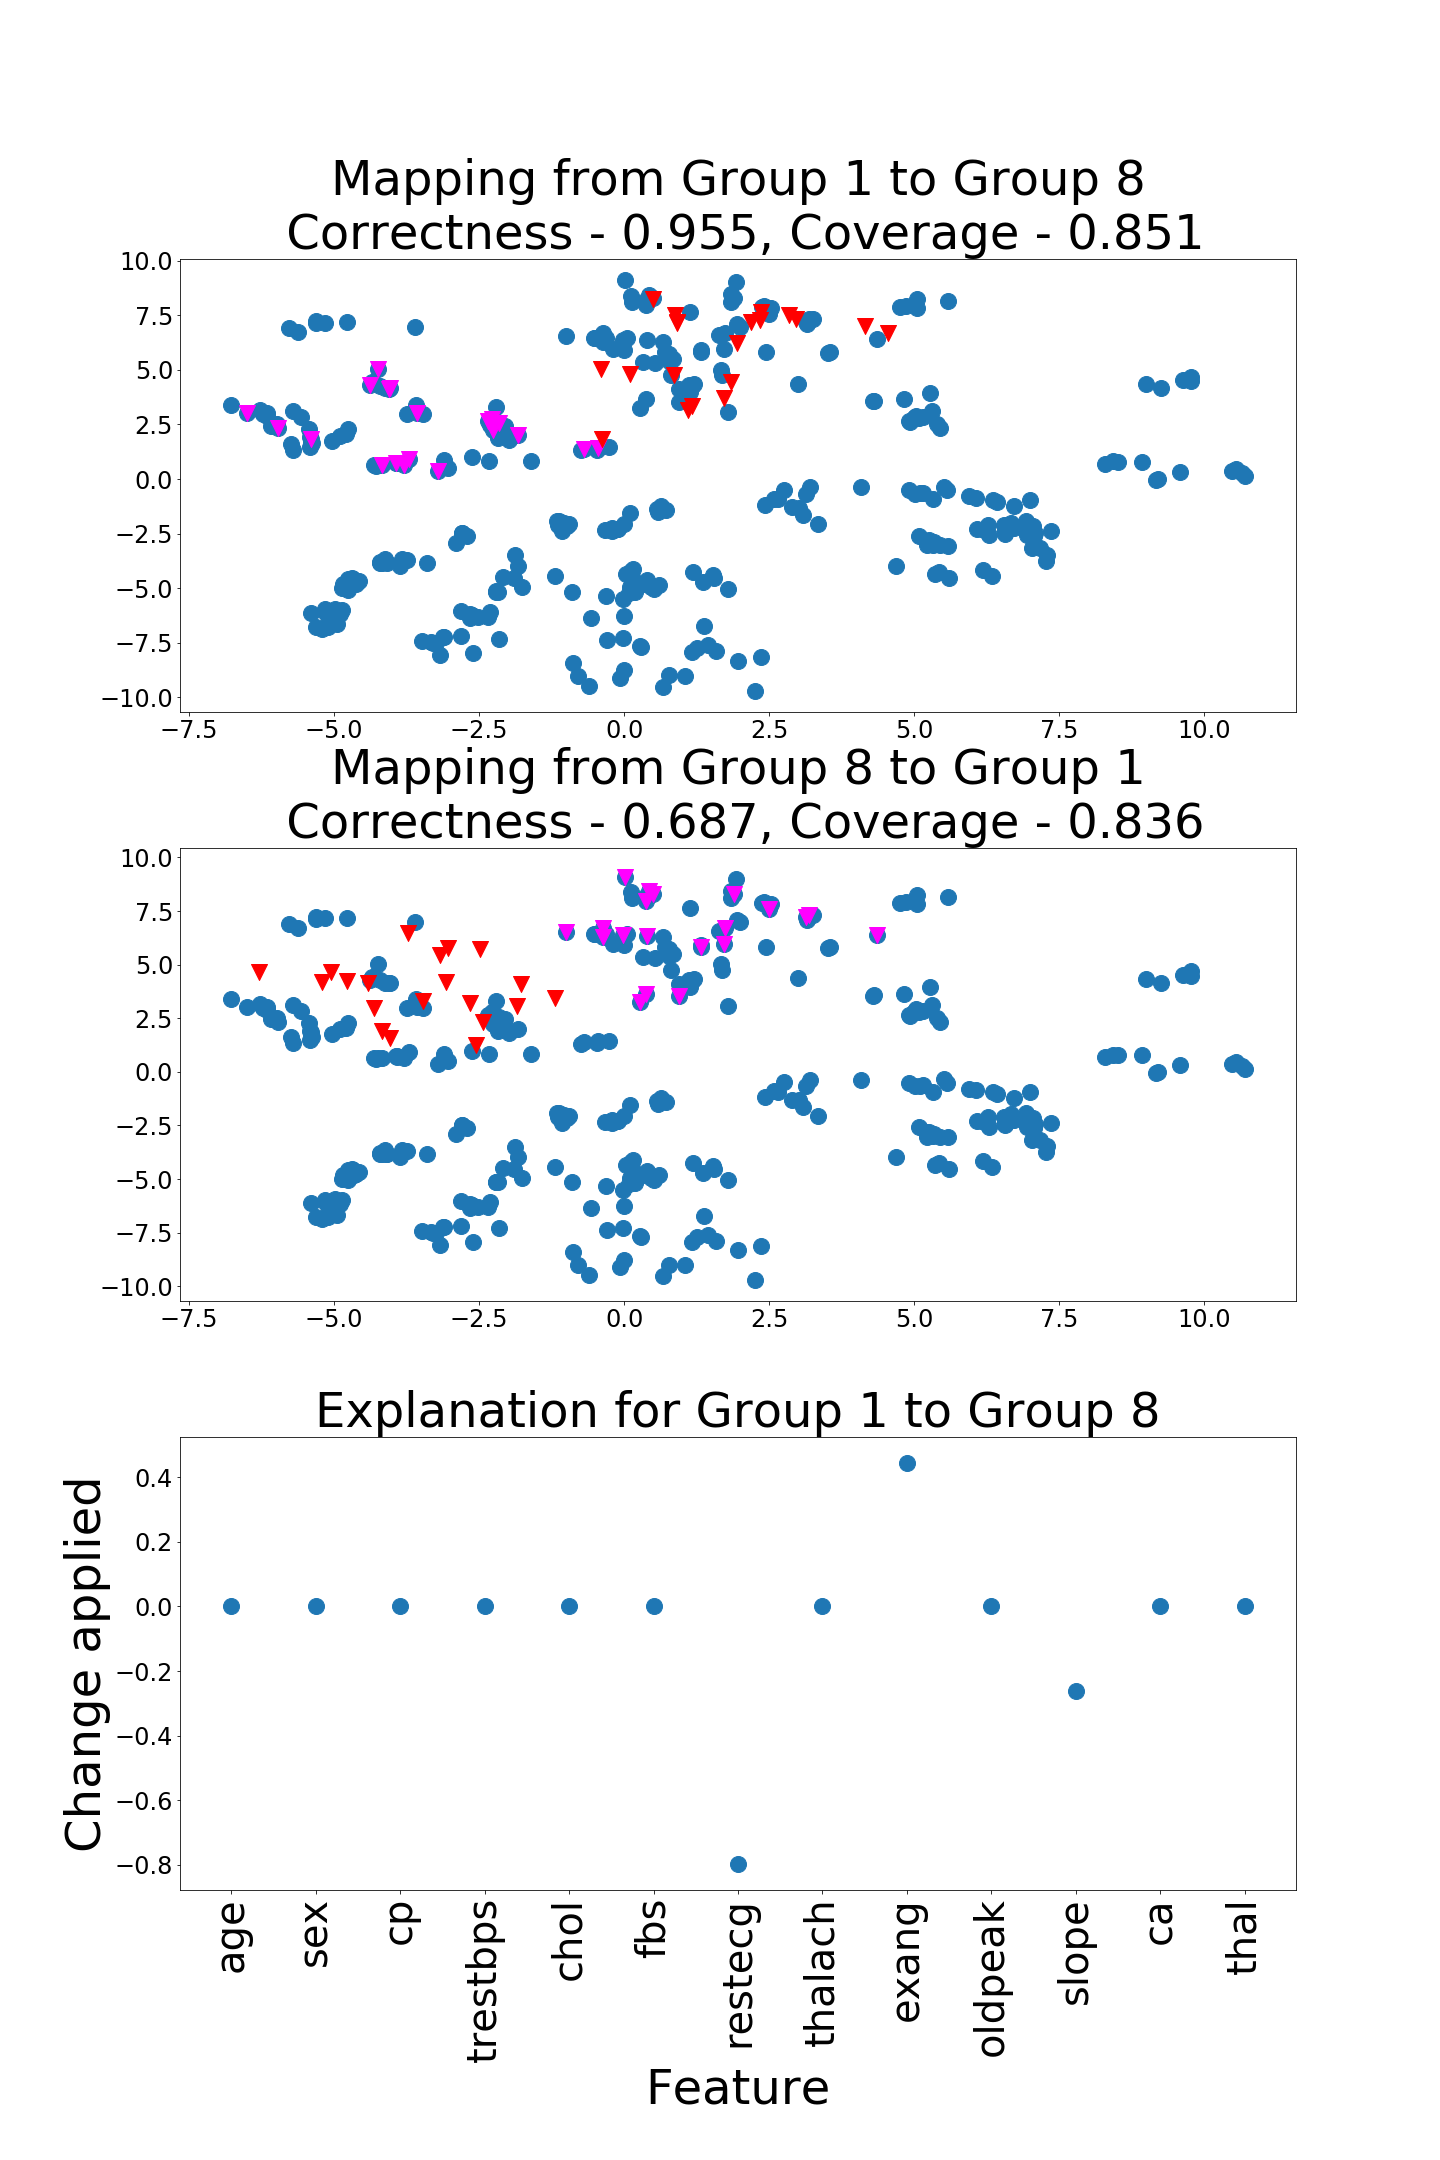
\includegraphics[width=0.4\textwidth, height=7.2cm]{../openreview/images/tffigures/heart-retrained-t2c.png}
    \caption{Explanation for corrupted features on UCI Heart Disease dataset. Left: Visualization of the TGT explanations on the modified dataset. We modified the 6(restecg) and 8(exang). However, the TGT recovers modifications in features 2(cp), 5(fbs), and 10(slope) instead. Right: Visualization of the TGT explanations with scVIS retrained on the modified dataset. With retrained scVIS model, TGT recovers the modified features along with 10(slope) feature. This observation does not entirely support the claim 4.}
    \label{fig:t2c-Heart}
\end{figure}
\subsection{Synthetic data}
\begin{figure}[H]
    \centering
    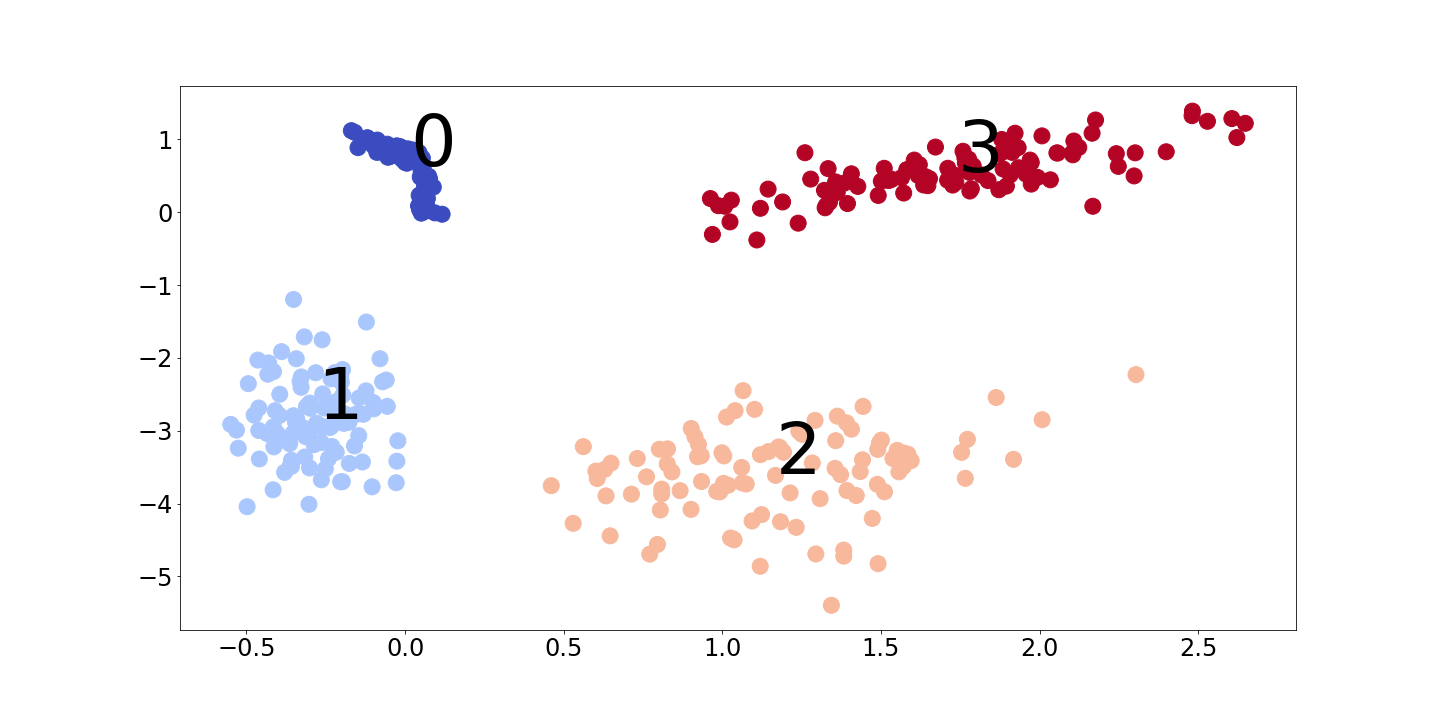
\includegraphics[width=0.4\textwidth, height=3cm]{../openreview/images/synthetic/synth-rep.png}
    % \hfill
    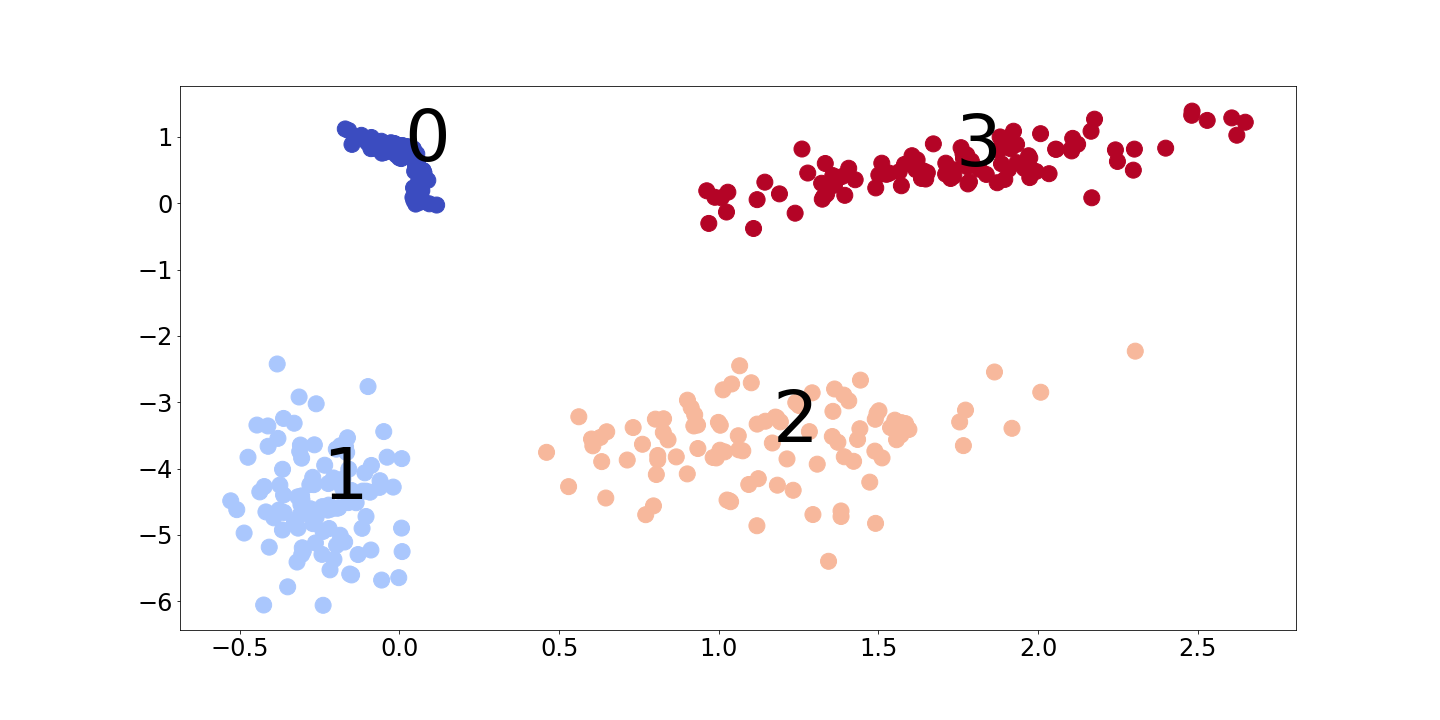
\includegraphics[width=0.4\textwidth, height=3cm]{../openreview/images/synthetic/modified.png}
    \caption{a) Synthetic data b) Synthetic data with the modification applied. We modify the data from group 1 across the $0^{th}$ dimension by $ax_{1}^{0} + b$. Here a and b are 2.0, 0.60 respectively.}
    \label{fig:synth_modified}
\end{figure}

\begin{figure}[H]
    \centering
    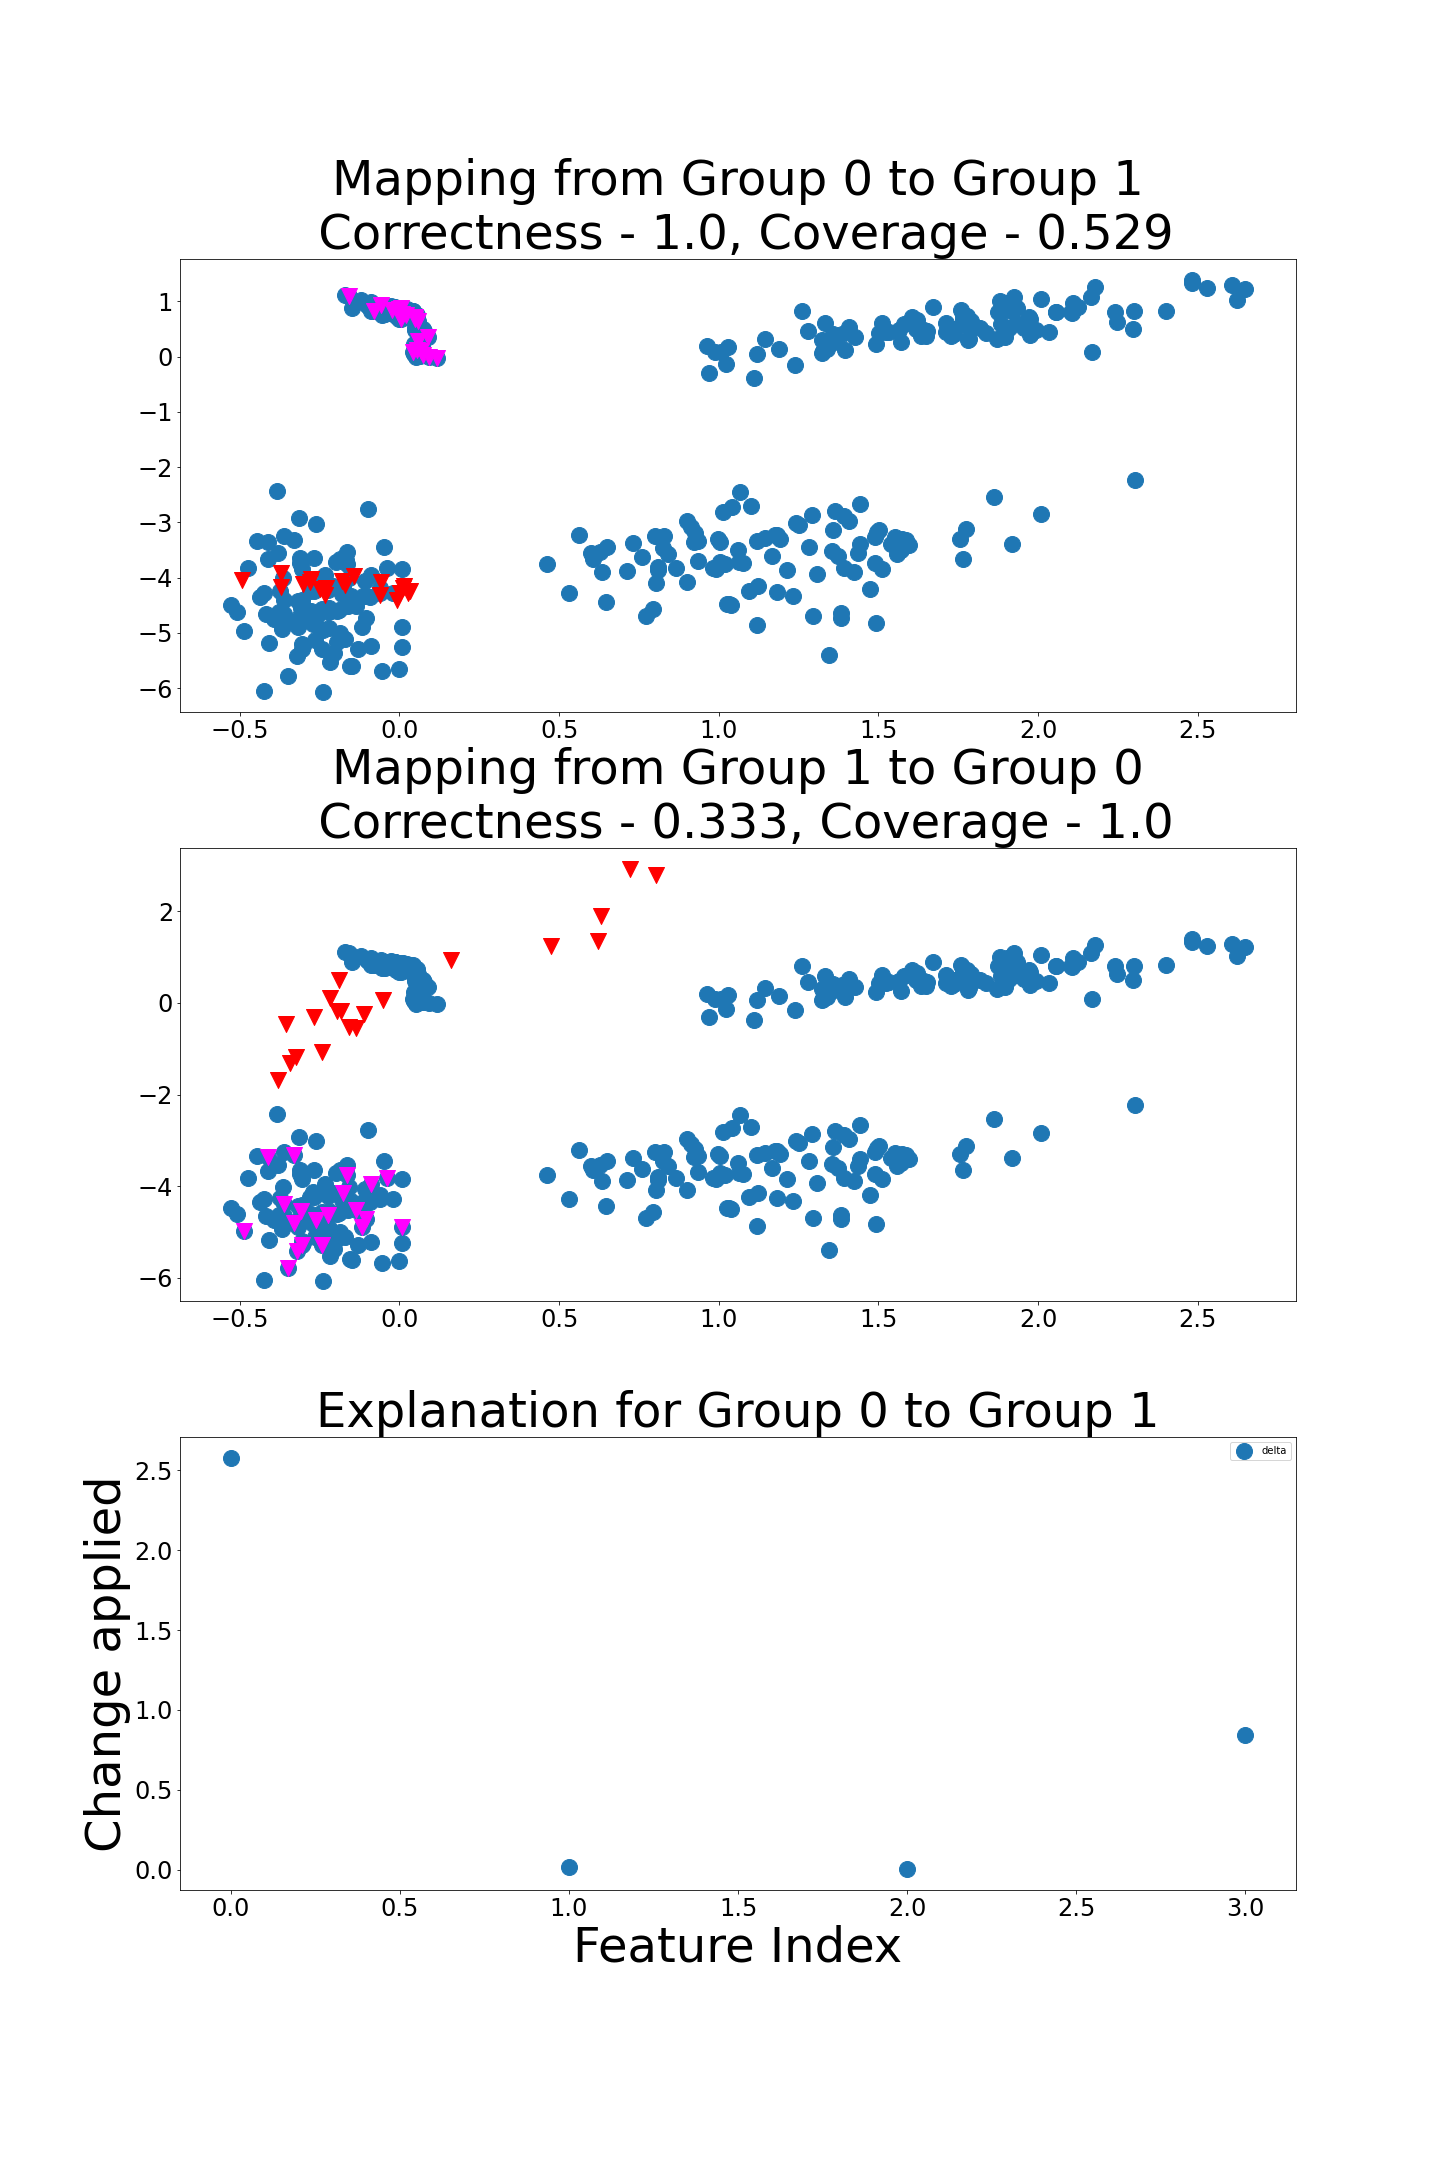
\includegraphics[width=0.4\textwidth, height=7.2cm]{../openreview/images/synthetic/synthetic_modified.png}
    % \hfill
    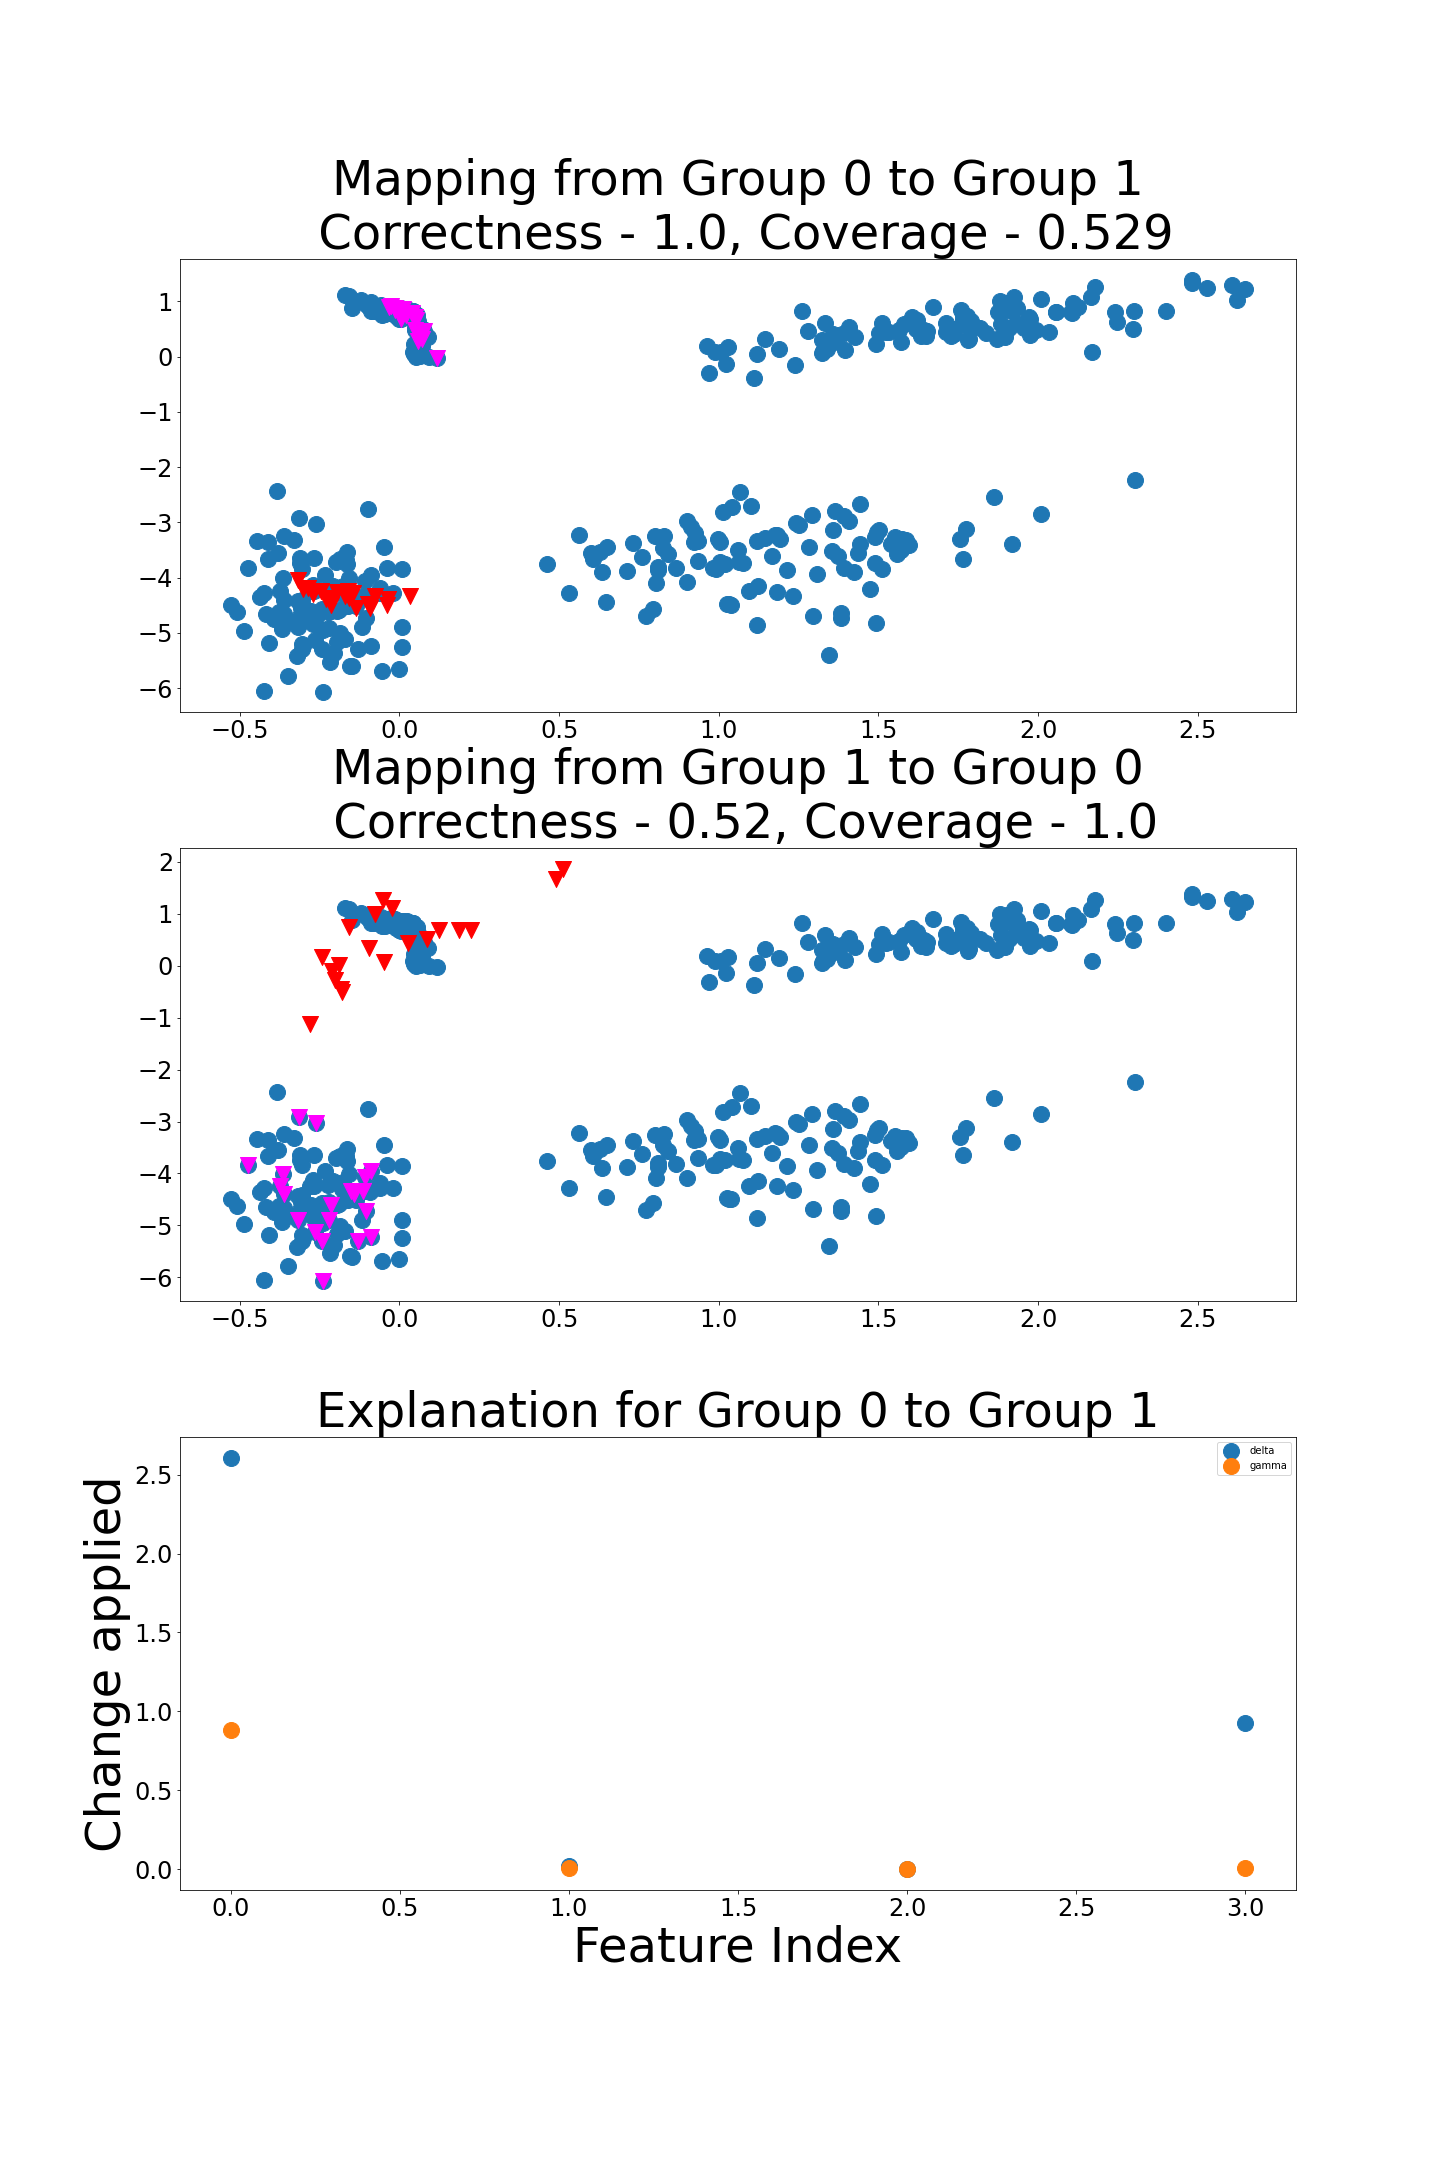
\includegraphics[width=0.4\textwidth, height=7.2cm]{../openreview/images/synthetic/synthetic_modified_scaling.png}
    \caption{We compare the explanations from the TGT algorithm (left) and the TGT with scaling extension algorithm(right) on the modified synthetic data. We can observe that the TGT with scaling extension has better correctness, and is able to identify the scaling we have applied across the first dimension (i.e. k=0). The $\gamma$ for this dimension is 0.87, which means the scaling factor is $e^{\gamma} \approx 2.38$. Moreover, the translation parameters are approximately same in both the variants of the TGT. }
    \label{fig:synth_modified_change}
\end{figure}
\newpage
\subsection{Probing Classifier and Feature Importance}
\label{app:dc}
\begin{figure}
    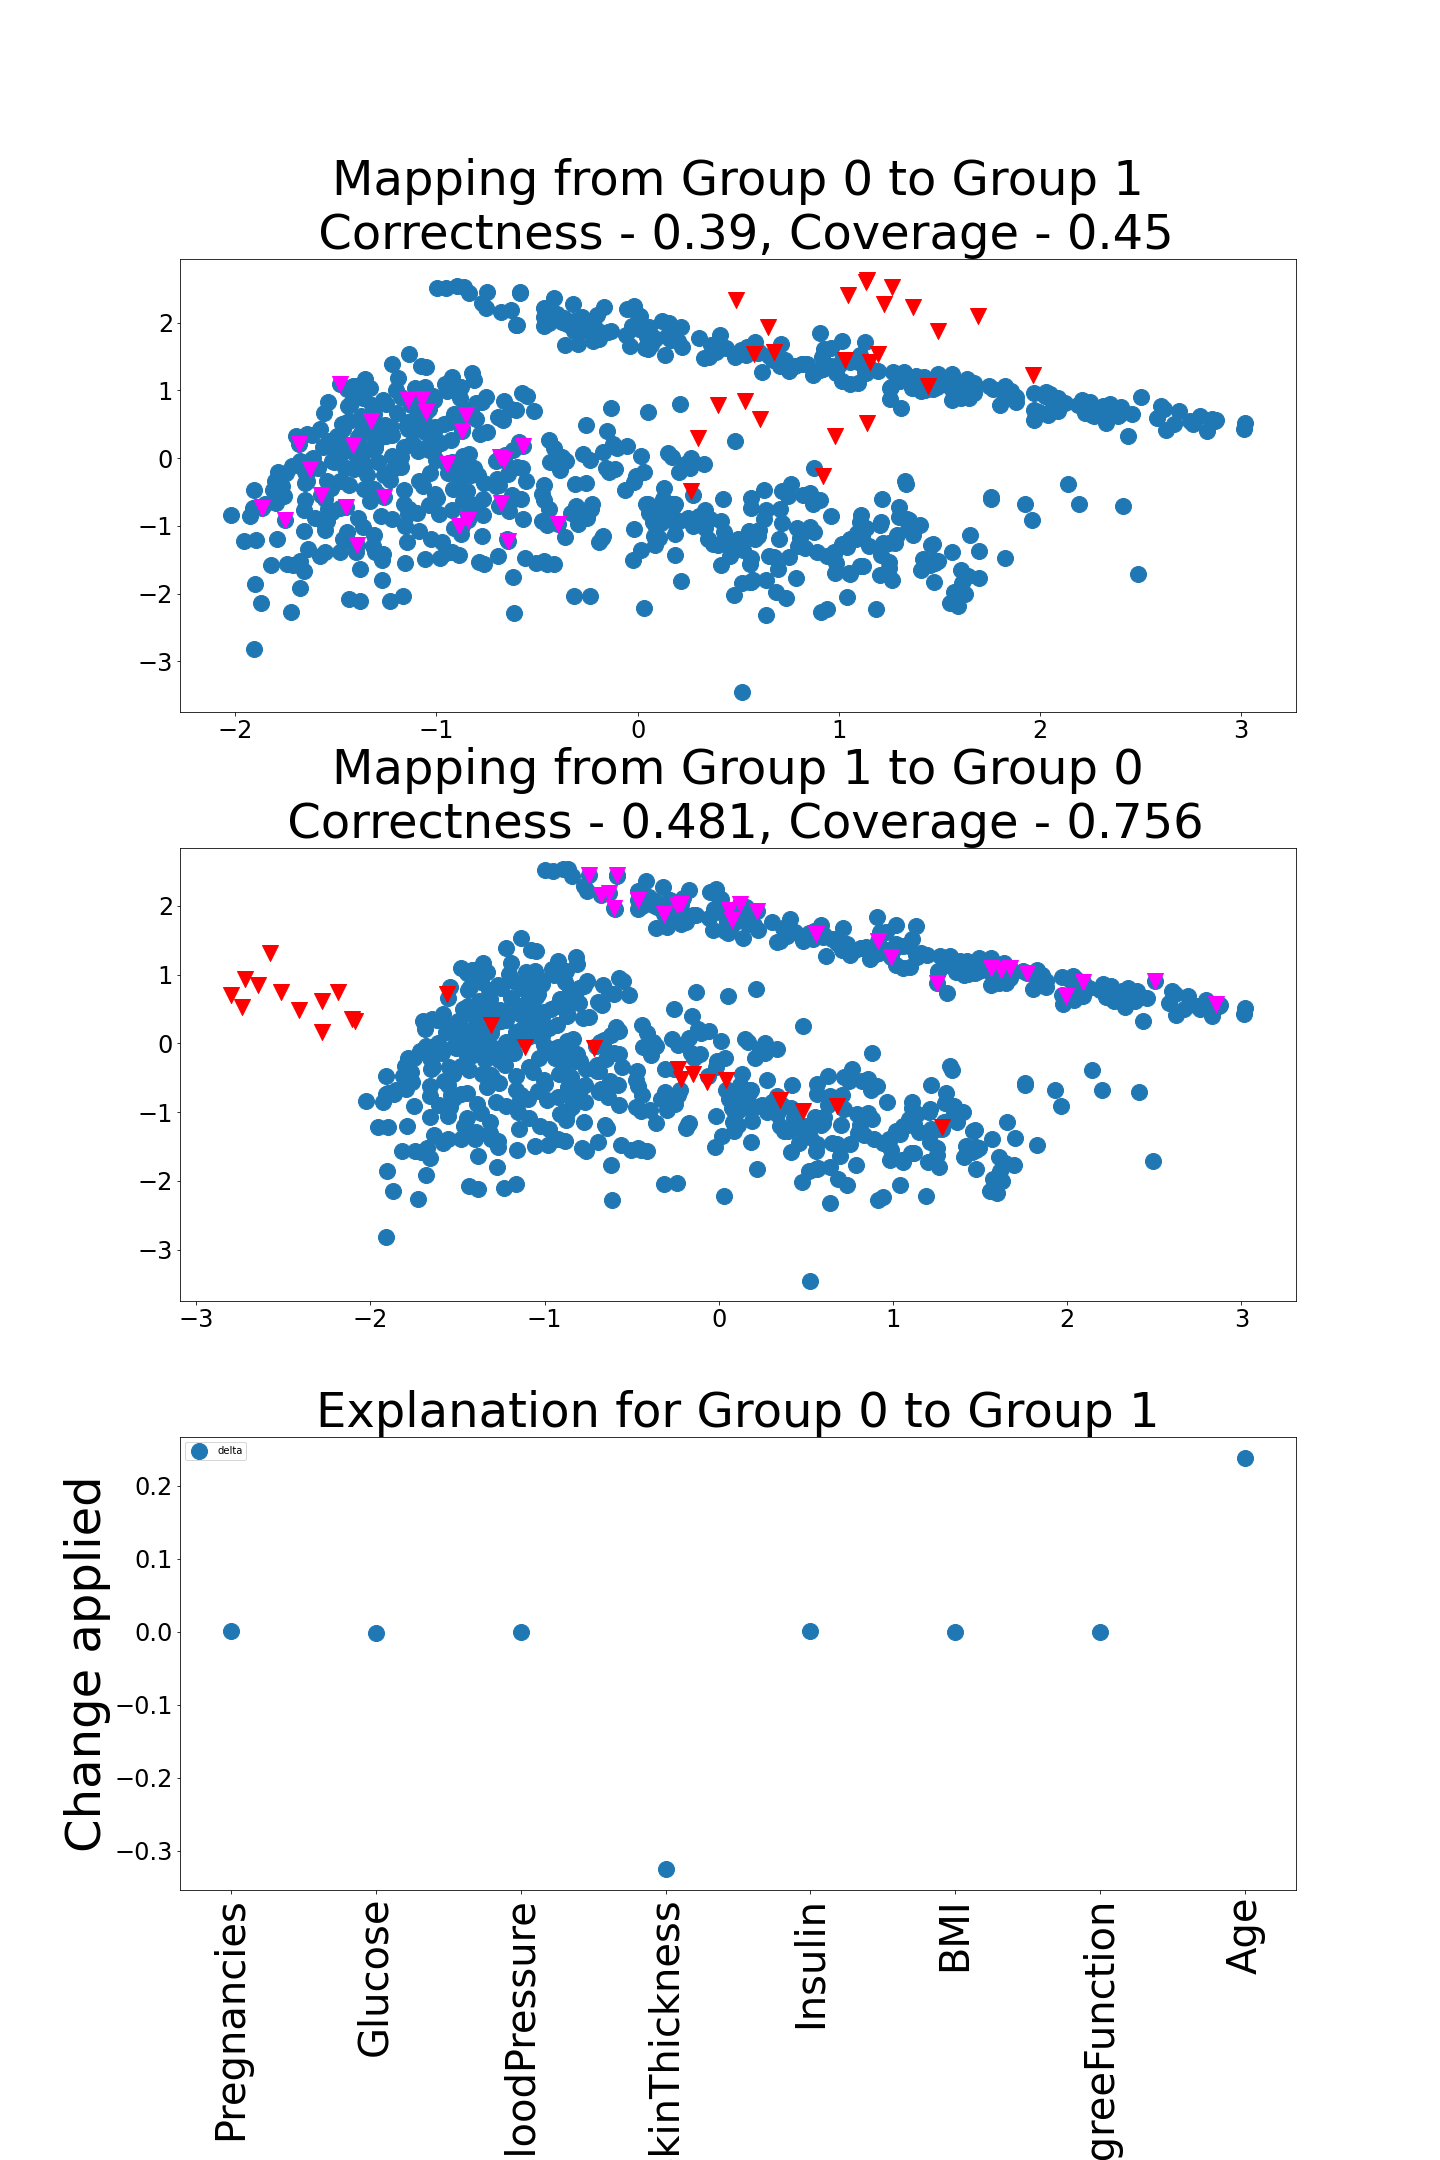
\includegraphics[width=0.4\textwidth, height=7.2cm]{../openreview/images/diabetes/diabetes-0to1.png}
    % \hfill
    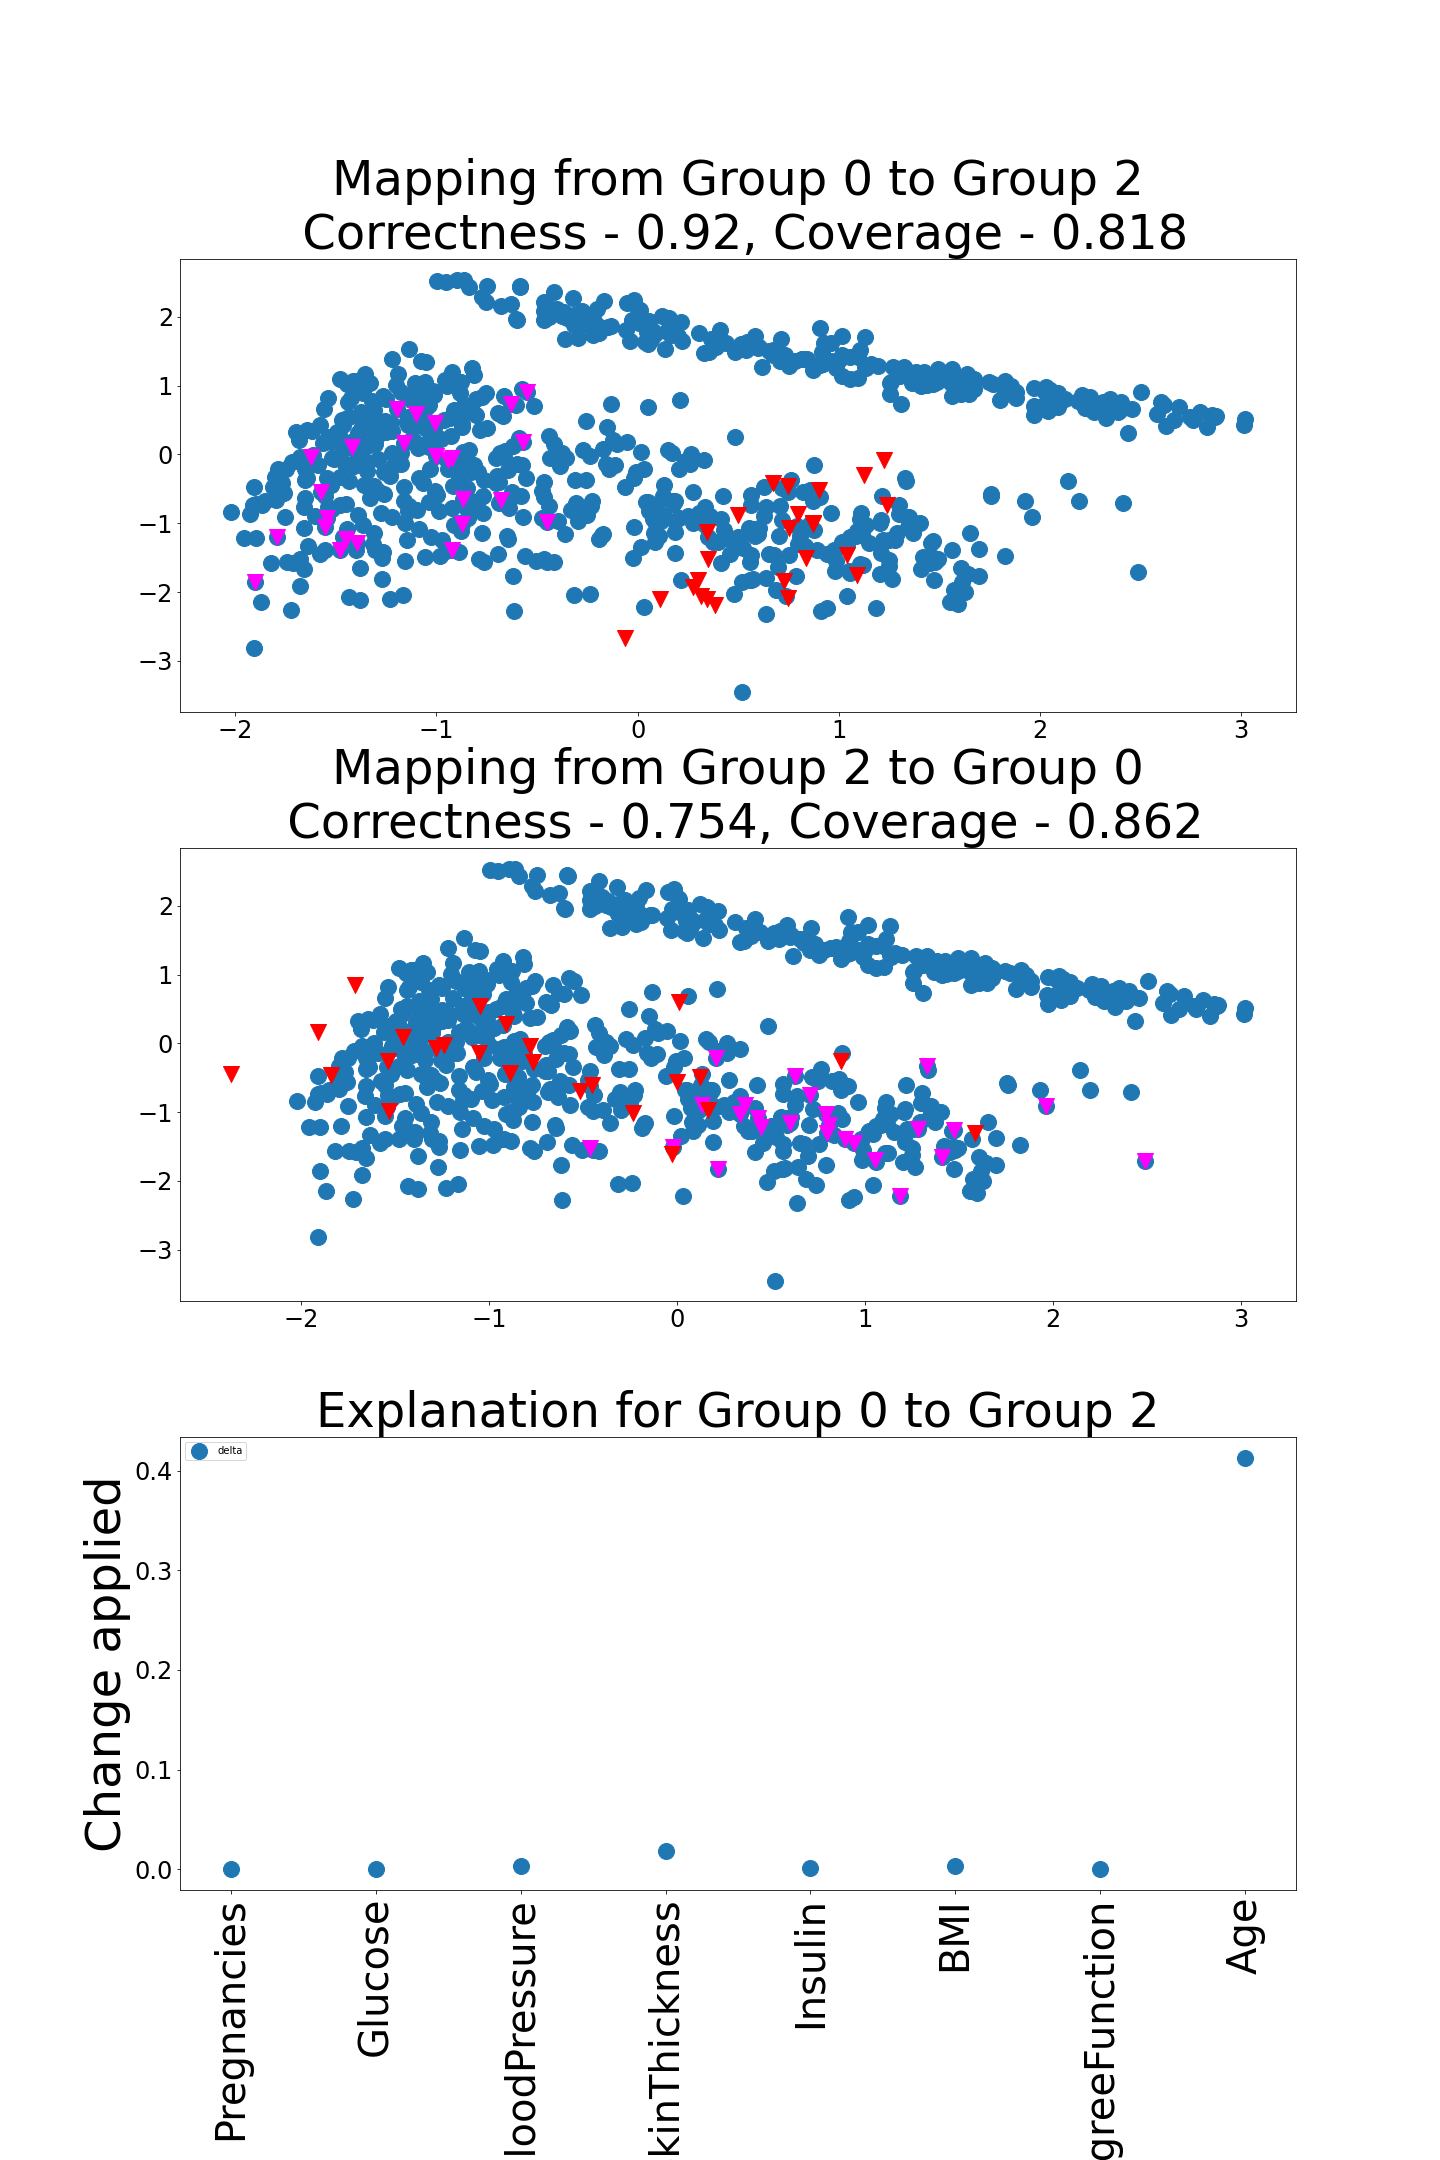
\includegraphics[width=0.4\textwidth, height=7.2cm]{../openreview/images/diabetes/diabetes-0to2.png}
    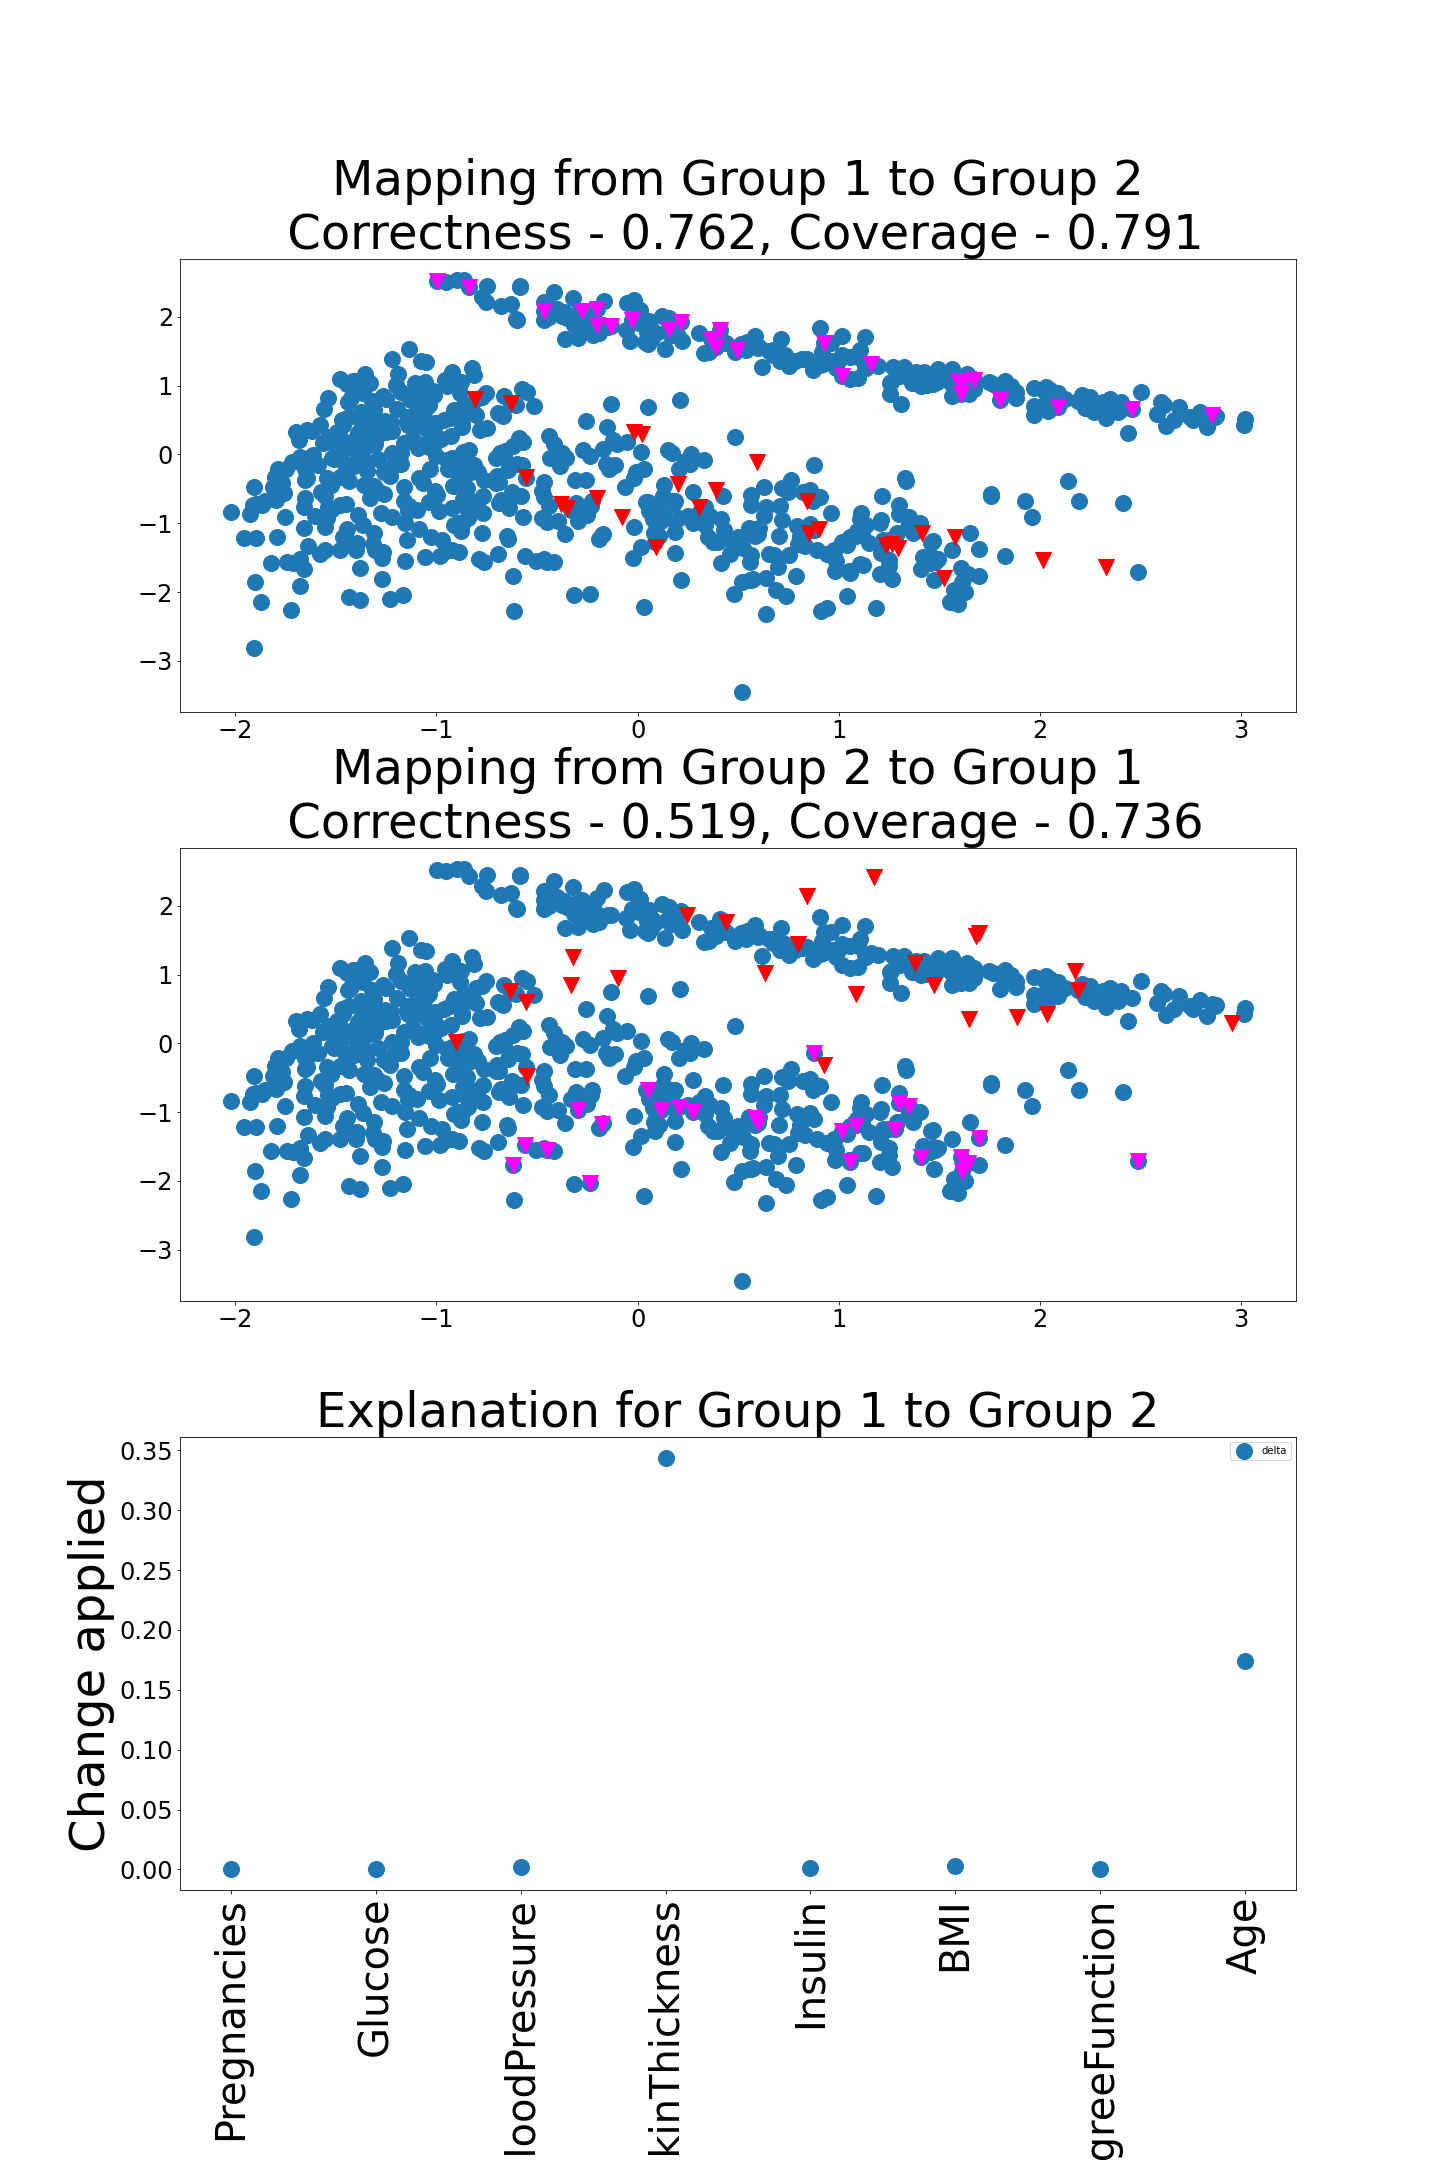
\includegraphics[width=0.4\textwidth, height=7.2cm]{../openreview/images/diabetes/diabetes-1to2.png}
    \caption{Explanations between different groups for the Pima Indians Diabetes Database.}
    \label{fig:diabetes_0}
\end{figure}
\begin{figure}
\centering
    \centering
     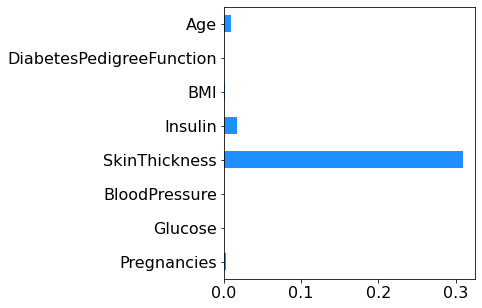
\includegraphics[width=0.4\textwidth, height=4cm]{../openreview/images/diabetes/0_.png}
     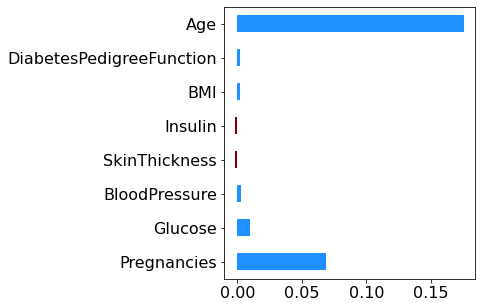
\includegraphics[width=0.4\textwidth, height=4cm]{../openreview/images/diabetes/1_.png}
      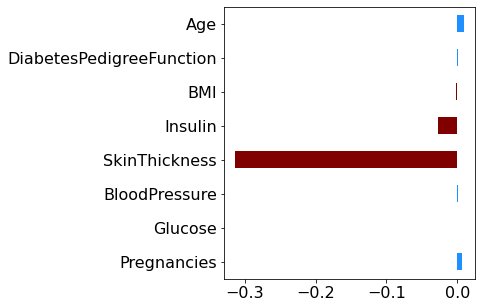
\includegraphics[width=0.4\textwidth, height=4cm]{../openreview/images/diabetes/2_.png}
    \caption{Feature Importance by the binary classifier for the Pima Indians Diabetes Database. a) (top-left): Feature importance for the classifier between groups 0 and 1. b) (top-right): Feature importance for the classifier between groups 0 and 2. c) (bottom-left): Feature importance for the classifier between groups 1 and 2. We note that the classifiers give significant feature importances to the features which correspond to the deltas (refer fig. \ref{fig:diabetes_0}).}
    \label{fig:diabetes_1}
\end{figure}